\documentclass[11pt,a4paper]{article}

\usepackage[T1]{fontenc}
\usepackage[utf8]{inputenc}
\usepackage[english]{babel}
\usepackage[a4paper,margin=25mm]{geometry}
\usepackage{amsmath,amssymb,amsthm}
\usepackage{graphicx}
\usepackage{booktabs}
\usepackage{multirow}
\usepackage{longtable}
\usepackage{array}
\usepackage{microtype}
\usepackage{xcolor}
\usepackage[hidelinks,colorlinks=false]{hyperref}
\usepackage{enumitem}
\usepackage{caption}

\captionsetup[table]{skip=4pt,labelfont=bf}
\captionsetup[figure]{skip=4pt,labelfont=bf}

% Relax float placement so large tables take a float page near their
% discussion instead of cascading to the end of the document.
\usepackage{placeins}
\setcounter{topnumber}{4}
\setcounter{bottomnumber}{2}
\setcounter{totalnumber}{6}
\renewcommand{\topfraction}{0.92}
\renewcommand{\bottomfraction}{0.85}
\renewcommand{\textfraction}{0.06}
\renewcommand{\floatpagefraction}{0.65}

\graphicspath{{figs/}}

\newtheorem{proposition}{Proposition}
\newtheorem{hypothesis}{Empirical Hypothesis}
\newtheorem{corollary}{Corollary}

\title{\textbf{SHARD: cell-keyed residual splitting for
alignment-resistant private dense retrieval}}
\author{Sergey M.\ Kurilenko\\
\small Moscow Institute of Physics and Technology\\
\small \texttt{kurilenko.sm@phystech.edu}}
\date{\today}

\begin{document}
\maketitle

\begin{abstract}
\noindent
Dense embeddings underpin semantic search and Retrieval-Augmented
Generation, yet a leaked vector store reveals much of the underlying text.
The dominant modern attacks---few-shot alignment, zero-shot inversion and
unsupervised cross-space translation---all exploit the same weakness: the
protected store is a \emph{single global geometry} that can be aligned to a
known space. A secret global rotation, the usual lightweight defence, falls
to orthogonal Procrustes once the attacker has on the order of the subspace
dimension in known plaintext pairs. We measure this baseline and then
introduce a transform built to remove its weak axis.

\textsc{Shard} is a family of retrieval-preserving embedding transforms.
The centred embedding is rotated and split into a short \emph{public}
prefix (used for coarse stage-1 retrieval) and a \emph{private} residual
that is sharded into $C$ coarse cells, each rotated by its own secret
orthogonal key; the residual is reranked under CKKS, where the per-cell
keys cancel and preserve the exact inner product. A single parameter $C$
interpolates between the global-linear baseline ($C{=}1$) and
per-document micro-keys ($C{=}N$). On cached embeddings from five encoders
we find: \textbf{(i)~utility}---because reranking is full-dimensional,
\textsc{Shard} recovers the raw quality that the truncating baseline loses,
including the nDCG@10 that half-SVD truncation drops on BEIR (e5-base/
SciFact: $0.638$ vs.\ raw $0.637$ vs.\ baseline $0.585$);
\textbf{(ii)~alignment resistance}---recovering the private residual into
the native frame under a \emph{diffuse} known-plaintext leak requires
$\approx\!C\times$ more anchors ($m_{50}$ rises from $200$ for a global key
to $102{,}400$ for $C{=}256$, reproduced on a second encoder), at a measured
cost of $\approx\!7$--$30$ encrypted residual queries per search;
\textbf{(iii)~public-index leakage}---the short prefix reveals far less
neighbour structure than the baseline's half-space (NN-overlap@10
$0.20$--$0.55$ vs.\ $0.76$), and the per-document micro-key limit drives the
residual graph leak to zero with an unlinkable, renewable template. The
barrier is not a Procrustes artefact: learned-linear (\textsc{ALGEN}-core),
non-linear and unsupervised (\textsc{vec2vec}-core) attackers do no better,
and at matched utility a distortion-aware DP-noise defence leaves
de-anonymisation R@1 near $1.0$ where \textsc{Shard} gives $0.0$.
We are equally explicit about the limits: cell-level keys leave within-cell
similarities and a $\approx\!C\times$ query-cost trade-off; a \emph{targeted}
attacker who concentrates anchors in a victim's (public) cell needs only
$\approx\!d_{\mathrm{priv}}$ anchors; and an \emph{overlapping} reference
corpus still de-anonymises through the public prefix. \textsc{Shard} hardens
the diffuse alignment/inversion surface, not the coarse graph; it is an
attack-aware geometric defence, not a cryptographic guarantee.
\end{abstract}

\textbf{Keywords:}
dense retrieval, embedding privacy, protective transforms, alignment
attacks, embedding inversion, cell-keyed splitting, cancellable templates,
homomorphic encryption, CKKS, retrieval-augmented generation.

% =====================================================================
\section{Introduction}
% =====================================================================

The privacy of vector representations of text---``embeddings''---has become
a first-class concern in production retrieval systems. Dense retrievers
(DPR \cite{ref_dpr}, ColBERT \cite{ref_colbert}) and state-of-the-art
encoders (Sentence-BERT \cite{ref_sbert}, multilingual-E5 \cite{ref_e5},
GTR \cite{ref_gtr}, BGE-M3 \cite{ref_bgem3}) push the per-document
representation through a
$\sim 10^2$-dimensional bottleneck that nevertheless preserves enough
information to reconstruct the original text with high BLEU.
\textsc{Vec2Text} \cite{ref_vec2text} reports
$\mathrm{BLEU} \approx 97.3\%$ on $32$-token inputs when the attacker has
query access to the encoder; \textsc{GEIA}~\cite{ref_geia} and
\textsc{TEIA}~\cite{ref_teia} show that even snapshot attacks
(an adversary with read access to the vector database) recover personally
identifiable information at high rates. For Retrieval-Augmented Generation
pipelines whose vector stores typically contain customer support tickets,
internal corporate documents and personal data, this rule of thumb---``a
leak of the embedding is a leak of the text''---is now well documented
\cite{ref_rag,ref_zeng_rag}.

The defensive landscape is bracketed by two extremes that, individually,
do not satisfy industrial requirements. Differential privacy
\cite{ref_dwork,ref_dpsgd} adds calibrated noise per-record but, in the
naive coordinate-Gaussian formulation on retrieval-quality embeddings, it
faces a difficult operating-point choice: mild noise preserves much of the
nearest-neighbour geometry, while stronger noise destroys ranking quality
long before the privacy budget reaches a level considered useful.
Fully homomorphic encryption \cite{ref_ckks,ref_openfhe}
allows arbitrary computation on ciphertexts, but the
ciphertext-ciphertext (ct-ct) regime is too expensive for top-$k$ search
across $10^6$ documents.

\paragraph{The weak axis of global-linear defences.} Between the two
extremes sits a popular lightweight middle ground: compress the collection
onto a data-dependent SVD subspace, apply a single secret orthogonal
rotation, publish an approximate-nearest-neighbour (ANN) index, and rerank
the encrypted query under CKKS. We first measure this global-linear stack
and confirm that its protection lives on \emph{one weak axis}---the
protected store is a single globally-aligned geometry. Concretely
(Section~\ref{sec:experiments}): a known-plaintext orthogonal Procrustes
attack recovers the secret rotation with about $k=d/2$ anchors, after which
an overlapping reference corpus yields near-exact paragraph recovery
($99.8\%$ top-1); the public product-quantisation index preserves a mean
cosine of $0.95$ and $67\%$ of exact top-10 neighbours; and because the
rerank happens in the truncated half, the stack \emph{loses} retrieval
quality on real IR, dropping nDCG@10 by $2$--$8$ points on BEIR. These are
exactly the weaknesses that modern few-shot alignment \cite{ref_algen},
zero-shot inversion \cite{ref_zsinvert} and unsupervised cross-space
translation \cite{ref_vec2vec} attacks exploit: a single global map is, in
the end, alignable.

\paragraph{\textsc{Shard}: an attack-aware geometric transform.} We
introduce \textsc{Shard}, a family of retrieval-preserving protective
transforms designed against the alignment and index-leakage attack surface
rather than against a distortion surrogate such as $\sigma_{rec}$ (which,
as we and others show, is not a privacy metric). The construction
(Section~\ref{sec:shard}) keeps the CKKS/ct-pt machinery of the baseline
but replaces its single global geometry. The contributions are:

\begin{itemize}[leftmargin=18pt]
\item \emph{Construction.} We rotate the centred embedding and split it
into a short \emph{public} prefix $u$ (top-$d_{\mathrm{pub}}$ PCA, for
coarse stage-1 retrieval) and a \emph{private} residual $r$. The residual
is sharded into $C$ coarse cells defined by $u$, each rotated by its own
secret orthogonal key $H_c$ (a product of Householder reflections), giving
the stored shard $z_i = H_{c(i)} r_i$. Reranking is done under CKKS in the
residual space, where the orthogonal keys cancel
($\langle H_c r_q, z_i\rangle=\langle r_q, r_i\rangle$) and preserve the
\emph{exact} inner product. A single knob $C$ interpolates between the
global-linear baseline ($C{=}1$) and per-document micro-keys ($C{=}N$),
and gives revocability at cell granularity.
\item \emph{Utility: full-dimensional rerank recovers raw quality}
(Section~\ref{ssec:shard-utility}). Because reranking is full-dimensional,
\textsc{Shard} recovers the raw ranking that the truncating baseline loses.
On the BEIR tasks where half-SVD truncation significantly drops nDCG@10,
\textsc{Shard} matches raw (e5-base/SciFact $0.638$ vs.\ raw $0.637$ vs.\
baseline $0.585$) while exposing a public channel only a quarter to a half
the baseline's width.
\item \emph{Alignment resistance scales with $C$}
(Sections~\ref{ssec:shard-cost}--\ref{ssec:shard-align})---the headline
result, with its cost and caveats measured, not assumed. Under a
\emph{diffuse} known-plaintext leak, recovering the private residual into
the native frame grows $\approx C\times$: median anchors rise from $200$
(global key) to $25{,}600$ ($C{=}64$) and $102{,}400$ ($C{=}256$), and the
result reproduces on a second encoder. The cost is $\approx7$--$30$
encrypted residual queries per search (the short-list spans that many
cells); and a \emph{targeted} attacker who concentrates anchors in a
victim's public cell needs only $\approx d_{\mathrm{priv}}$ ($320$/$576$ on
our two encoders, vs.\ $1.7\times$ the baseline's $d/2$), so the $C\times$
gain is an aggregate/diffuse-leak property. The barrier survives stronger
attackers (Section~\ref{ssec:shard-learned})---the learned-linear core of
\textsc{ALGEN}, a non-linear MLP, and unsupervised \textsc{vec2vec}-style
matching all do no better than the orthogonal Procrustes we use---and
against a distortion-aware DP-noise baseline at matched utility
(Section~\ref{ssec:shard-vs-dp}), \textsc{Shard} alone reaches near-zero
de-anonymisation.
\item \emph{The public channel leaks coarse, not fine, structure, and
micro-keys remove the residual leak} (Sections~\ref{ssec:shard-leak},
\ref{ssec:shard-micro}). The short prefix reveals far less neighbour
structure than the baseline's exposed half (NN-overlap@10 from $0.20$ at
$d_{\mathrm{pub}}{=}d/16$ to $0.55$ at $d/4$, vs.\ $0.76$). The within-cell
residual graph the server can reconstruct shrinks with $C$ ($0.25$ at
$C{=}64$, $0.18$ at $C{=}256$) and reaches $0.00$ for per-document
micro-keys, which also give an unlinkable, renewable template
(re-keying AUC $\approx0.5$).
\item \emph{Honest limitation} (Section~\ref{ssec:shard-ref}).
\textsc{Shard} hardens the diffuse native-frame mapping, not the coarse
graph: within a cell the keys cancel, and an \emph{overlapping} reference
corpus still de-anonymises through the public prefix once its single cheap
global key is recovered. We measure this and discuss the coarse-cell-ID and
micro-key variants that close it at a recall or bandwidth cost.
\end{itemize}

\noindent
The global-linear baseline characterisation (alignment, PQ leakage,
BEIR-truncation loss, and the calibrated-noise diagnostic that
$\sigma_{rec}$ is not a privacy metric) is retained in
Section~\ref{sec:experiments} as the foil that motivates \textsc{Shard},
together with the CKKS ct-pt speed-up and parameter selection
(Sections~\ref{ssec:ckks-modes},~\ref{sec:autotune}) that both schemes
share.

\paragraph{Notation.} To avoid the overloading of the symbol $N$, we use
$N_{\mathrm{poly}}$ for the CKKS polynomial-modulus degree,
$N_{\mathrm{docs}}$ for the corpus size, and $K_{\mathrm{cands}}$ for the
stage-1 short-list length throughout.

\paragraph{An elementary proxy bound.} We state a one-line projection
bound (Proposition~\ref{lemma:proj-l2}): any decoder whose image is
constrained to $\mathrm{span}(V_k)$ has $L_2$ reconstruction error at
least $\|\mathbf{x}_\perp\|_2$. This is a Pythagorean fact, not a security
theorem; we use it only to make $\sigma_{rec}$ a precise distortion proxy
within that decoder class. Its empirical relation to the BLEU of an
off-the-shelf \textsc{Vec2Text} attack is reported as Empirical
Hypothesis~\ref{hyp:bleu}.

\paragraph{Roadmap.} Section~\ref{sec:related} reviews related
literature; Section~\ref{sec:threat} states the threat model;
Section~\ref{sec:method} describes the global-linear baseline (the foil)
and the shared CKKS/ct-pt machinery;
Section~\ref{sec:autotune} the CKKS parameter selection;
Section~\ref{sec:lemma} an elementary projection bound;
Section~\ref{sec:shard} introduces \textsc{Shard};
Section~\ref{sec:experiments} reports the baseline characterisation and the
four \textsc{Shard} experiments (utility, alignment resistance,
public-index leakage, and the reference-lookup limitation);
Section~\ref{sec:discussion} discusses limitations and open work.

% =====================================================================
\section{Related Work}\label{sec:related}
% =====================================================================

\paragraph{Embedding inversion.} \textsc{Vec2Text} \cite{ref_vec2text}
trains an encoder--decoder model that iteratively rewrites a candidate
hypothesis until its embedding matches a target vector; on
$32$-token \textsc{MS-MARCO} inputs the attack achieves
$\mathrm{BLEU} \approx 97.3\%$ and $\approx 92\%$ exact recovery.
\textsc{GEIA} \cite{ref_geia} relaxes the discreteness of the input by
operating in the continuous embedding space and back-transcribing.
\textsc{TEIA} \cite{ref_teia} extends the threat model to
training-data extraction. Earlier work of Song and
Raghunathan~\cite{ref_song_leak} already established that embedding models
leak substantial information about their inputs. Adjacent work on
membership-inference \cite{ref_shokri} and on extracting training
texts from large language models \cite{ref_carlini} confirms that the
risk surface of dense retrievers is broader than the embedding-inversion
literature alone suggests. The 2025 generation of attacks further
weakens any defence that relies only on an unknown embedding orientation:
\textsc{ALGEN} aligns a victim embedding space to an attack space with
few known pairs and then generates text \cite{ref_algen};
\textsc{ZSInvert} removes the need for an embedding-specific inversion
model by using a universal zero-shot decoding strategy
\cite{ref_zsinvert}; and \textsc{LAGO} extends few-shot inversion to
cross-lingual settings by coupling alignments across related languages
\cite{ref_lago}. These papers motivate the alignment experiment in
Section~\ref{ssec:alignment-pq}: if a secret rotation can be absorbed by
a small alignment matrix, it must not be described as a security
guarantee.

\paragraph{Lightweight defences and transformed representations.}
Recent defences increasingly treat embeddings as representations whose
geometry can be compressed, transformed or regularised rather than merely
noised. \textsc{EGuard} uses a projection network with mutual-information
regularisation to reduce inversion leakage \cite{ref_eguard};
\textsc{SPARSE} studies concept-aware privacy mechanisms and anisotropic
noise for embedding inversion resistance \cite{ref_sparse}; and
nonparametric variational DP work adds bottleneck/noise mechanisms at
the representation level \cite{ref_nvdp}. Matryoshka-style representation
learning shows that retrieval utility can be deliberately concentrated in
prefix subspaces \cite{ref_mrl}, while recent cross-space translation
work argues that embedding spaces share enough geometry for transfer
maps to be useful \cite{ref_vec2vec}. \textsc{Shard} builds on both
observations: it uses a Matryoshka-style prefix as a deliberately coarse
public channel, precisely because the cross-space-translation literature
shows that a single global geometry is alignable.

\paragraph{Cancellable templates and decoupled encoders.}
\textsc{Shard}'s cell-local keys import two ideas that are standard in
biometric template protection but rare in text retrieval. Cancellable
biometrics \cite{ref_cancellable} require a protected template to be
\emph{renewable} (re-key after compromise) and \emph{unlinkable} (the same
identity under two keys should not be matchable); a product of secret
Householder reflections per cell gives \textsc{Shard} both at cell
granularity. Separately, work on retrieval with asymmetric
document/query encoders \cite{ref_dpr,ref_colbert} shows that the
document and query sides need not share one geometry---the structural
premise that lets \textsc{Shard} key the stored side while keeping queries
encrypted. Our contribution is to combine a coarse public prefix, a
cell-keyed private residual, and CKKS reranking into one
retrieval-preserving transform, and to show \emph{measured} advantages on
the alignment and index-leakage attack surface relative to the
global-linear baseline.

\paragraph{Differential privacy for embeddings.} Lyu et al.~\cite{ref_lyu}
investigate per-coordinate Gaussian noise on dense representations; the
empirical finding is that retrieval quality degrades sharply long before
$\varepsilon$ reaches a useful range. Random-projection-based privacy
\cite{ref_liu,ref_kenthapadi} predates modern dense retrieval; the
data-dependent SVD projection used here is closer to a noise-removal
technique than to a privacy-preserving DP mechanism, although
$\sigma_{rec}$ provides a useful proxy quantity.

\paragraph{Homomorphic encryption.} The CKKS scheme~\cite{ref_ckks}
introduced approximate-arithmetic FHE; OpenFHE \cite{ref_openfhe} and
TenSEAL provide production-grade implementations.
The bootstrapping cost \cite{ref_ckks_bootstrap} pushes practitioners
to leveled circuits; specialised compilers \cite{ref_eva,ref_chet}
optimise scale and modulus chains.
GPU acceleration of CKKS bootstrap \cite{ref_jung_gpu} and Intel HEXL
\cite{ref_hexl} have made larger leveled circuits feasible.

\paragraph{Hybrid privacy-preserving retrieval.} Tiptoe \cite{ref_tiptoe}
combines clustering with PIR for query privacy. SealPIR
\cite{ref_sealpir}, OnionPIR \cite{ref_onionpir} and SimplePIR
\cite{ref_simplepir} provide single-server PIR with practical query sizes.
The architecture in this paper is complementary: ct-pt CKKS reranking
takes care of the value side of the leakage, while access patterns
remain a separate problem for which PIR/ORAM-like primitives are an
appropriate composition.

% =====================================================================
\section{Threat Model}\label{sec:threat}
% =====================================================================

The global-linear baseline and \textsc{Shard} share one threat model, which
we fix here. It is asymmetric---a \emph{trusted client} (the data owner), an
\emph{honest-but-curious server}, and a \emph{non-adaptive} baseline
attacker, strengthened by the \emph{known-plaintext} attacker we use
throughout the alignment analysis. This is a fat-client, data-owner setting:
the client runs the encoder, holds all keys, performs stage-1 retrieval
locally, and the server only reranks under CKKS---a scoping assumption, not
the only possible deployment. Tables~\ref{tab:threat} and~\ref{tab:claims}
map the \emph{baseline}'s coverage and claims (the foil);
Table~\ref{tab:shard-claims} does the same for \textsc{Shard} (the
contribution, Section~\ref{sec:shard}).

\begin{itemize}[leftmargin=18pt,topsep=4pt,itemsep=2pt]
\item The \emph{client} is the data owner. It runs the encoder $E$,
generates the secret keys $\mu, V_k, R, sk_{\mathrm{CKKS}}$ and never
shares them. The client is trusted in software and key management.
\item The \emph{server} runs the search service over the rotated database
$E_{\mathrm{rot}} \in \mathbb{R}^{N_{\mathrm{docs}} \times k}$ and the
public PQ artefact. It is honest-but-curious: it follows the protocol but
attempts to extract textual information from the data it sees and from the
queries it processes.
\item The \emph{attacker} is, at minimum, non-adaptive (an off-the-shelf
\textsc{Vec2Text} model with no knowledge of $R$). Against both schemes we
additionally evaluate a known-plaintext alignment attacker (diffuse and, for
\textsc{Shard}, targeted), public-index leakage, reference-corpus lookup,
and---against \textsc{Shard}'s keyed residual---the learned-linear
(\textsc{ALGEN}) and unsupervised (\textsc{vec2vec}) alignment cores and a
non-linear MLP (Section~\ref{ssec:shard-learned}). Malicious server
behaviour and the full \emph{generative} stages of the modern inverters
remain out of scope.
\end{itemize}

\paragraph{Three distinct privacy notions.} A recurring source of
confusion in hybrid designs is the conflation of \emph{what} is
protected. We therefore separate three independent notions and state,
for each, exactly which component is responsible:

\begin{itemize}[leftmargin=18pt,topsep=4pt,itemsep=2pt]
\item \textbf{Document privacy.} The plaintext rotated database
$E_{\mathrm{rot}}$ \emph{is} visible to the server. It is protected only
by SVD truncation ($\sigma_{rec}$, a proxy quantity) and the secret
rotation $R$ (an empirical obfuscation layer). \emph{This is not a
cryptographic protection}; it fails under known-$R$ and, as
Section~\ref{ssec:alignment-pq} shows, under a modest
known-plaintext alignment attack.
\item \textbf{Query privacy.} CKKS hides the numerical value of the
query vector and of the similarity scores from the server. This part
\emph{is} cryptographic, at the chosen security level.
\item \textbf{Access-pattern privacy.} The candidate IDs reranked per
query, and the public PQ codes, are \emph{not} hidden. CKKS does not
address this channel; it requires composition with a PIR/ORAM-style
primitive.
\end{itemize}

In particular, the public PQ artefact (codebook + per-document codes,
trained in the rotated space) is itself a lossy compressed view of
$E_{\mathrm{rot}}$. Section~\ref{ssec:alignment-pq} quantifies this
leakage on a controlled sample; the result is strong enough that public
PQ codes must be treated as a meaningful side channel rather than as a
harmless index artefact.

Table~\ref{tab:threat} summarises the coverage and
Table~\ref{tab:claims} maps each claim to the evidence that supports it.
The diagonal of the coverage table is intentional: ct-pt reranking takes
care of the value channel, but the access-pattern channel (which document
IDs are reranked) remains open, and the public-PQ-artefact channel is
measured as leaky rather than closed. They would require composition with
a PIR-style primitive and a stronger static-side index protection,
respectively.

\begin{table}[tbp]
\centering
\caption{Threat coverage of the global-linear \emph{baseline} (the foil).
\textsc{Shard}'s coverage of the same vectors is in
Table~\ref{tab:shard-claims}.}\label{tab:threat}
\small
\begin{tabular}{@{}p{0.42\linewidth}p{0.10\linewidth}p{0.42\linewidth}@{}}
\toprule
\textbf{Attack vector} & \textbf{Covered?} & \textbf{Comment} \\ \midrule
Snapshot of $E_{\mathrm{rot}}$ without $R$ (off-the-shelf Vec2Text) &
Partial &
Heuristic; empirically validated against non-adaptive Vec2Text. \\
Network interception, leakage of similarity scores &
Yes &
CKKS at tc128; $sk$ never leaves the client. \\
Known $R$ (known-rotation attacker) &
No &
Reduces to $\sigma_{rec}$ from SVD truncation only. \\
Known-plaintext pairs $(\mathrm{text}_i, E_{\mathrm{rot},i})$ &
No &
Evaluated in Section~\ref{ssec:alignment-pq}; roughly $k$ pairs
recover the rotation numerically. \\
Reference-corpus overlap after known-plaintext alignment &
Partial &
Evaluated in Section~\ref{ssec:reference-attack}; overlapping texts are
recoverable. \\
Unsupervised cross-space translation attacks &
No &
Not evaluated on the baseline; the \textsc{vec2vec} alignment core
\emph{is} evaluated against \textsc{Shard}'s residual
(Section~\ref{ssec:shard-learned}). \\
Adaptive / learned alignment decoder &
No &
Sections~\ref{ssec:vec2text}, \ref{ssec:adaptive-inversion} use
off-the-shelf Vec2Text on the baseline; learned-linear/MLP alignment is
tested against \textsc{Shard} (Section~\ref{ssec:shard-learned}). \\
Malicious server (protocol deviation, substitution) &
No &
Verifiable computation / TEEs are an orthogonal addition. \\
Access-pattern leakage on candidate IDs &
No &
CKKS hides values, not access patterns; requires PIR/ORAM. \\
Leakage from the public PQ artefact (rotated-space codes) &
Partial &
Evaluated in Section~\ref{ssec:alignment-pq}; neighbour structure is
substantially preserved, so this remains an exposed channel. \\
\bottomrule
\end{tabular}
\end{table}

\begin{table}[tbp]
\centering
\caption{\emph{Baseline} claims vs.\ evidence (the foil): which statements
about the global-linear stack are demonstrated and which are deliberately
\emph{not} claimed. \textsc{Shard}'s claims are in
Table~\ref{tab:shard-claims}.}
\label{tab:claims}
\small
\begin{tabular}{@{}p{0.40\linewidth}p{0.54\linewidth}@{}}
\toprule
\textbf{Claim} & \textbf{Evidence / status} \\ \midrule
CKKS hides query values and scores from the server &
Cryptographic construction + parameters (Sec.~\ref{sec:autotune},
\ref{ssec:crypto-detail}); query privacy is cryptographic. \\
ct-pt is faster than ct-ct for the reranking &
Section~\ref{ssec:ckks-modes} ($1.44\times$ on the micro-benchmark,
$1.7\times$ at the auto-tuned configuration). \\
Secret rotation helps against \emph{off-the-shelf}, non-adaptive
Vec2Text & Section~\ref{ssec:vec2text}; effect holds only for the
tested weak-attacker configuration. \\
Aligned off-the-shelf Vec2Text recovers text/PII after Procrustes &
Section~\ref{ssec:adaptive-inversion}: \textbf{not observed} in the
memory-capped RTX~4090 run, but the raw baseline is also near the
reconstruction floor, so this is not a proof of security. \\
Secret rotation is robust to known-plaintext alignment &
\textbf{False}; Section~\ref{ssec:alignment-pq} shows near-exact
recovery with about $k$ known pairs. \\
Public PQ codes are harmless metadata &
\textbf{False}; Section~\ref{ssec:alignment-pq} shows substantial
reconstruction and nearest-neighbour leakage. \\
The protective wrapper preserves ranking in $\mathrm{span}(V_k)$ &
Section~\ref{ssec:integral} (within the 5-seed CI). \\
SVD truncation improves \emph{Acc@1} (a ``denoiser'') &
\textbf{Not significant}; Section~\ref{ssec:significance}: paired tests
give $p\geq0.11$ for every encoder. \\
SVD truncation significantly improves \emph{Acc@10} for $d{=}1024$
retrieval-trained encoders &
Section~\ref{ssec:significance} (e5-large $+0.042$, $p<10^{-6}$); it
significantly \emph{degrades} compact/paraphrase encoders. \\
The denoiser generalises to real IR &
\textbf{False}; Section~\ref{ssec:beir}: SVD significantly \emph{reduces}
nDCG@10 on BEIR SciFact/NFCorpus for every encoder. \\
$\sigma_{rec}$ alone measures document privacy &
\textbf{Not claimed}; Section~\ref{ssec:projection-baselines} shows that
matched-distortion noise can preserve substantially more raw neighbour
structure. \\
End-to-end query latency $<1$~s at $10^6$ docs &
Section~\ref{ssec:latency} (loopback PoC). \\
The system is secure against an \emph{adaptive} inversion attacker &
\textbf{Not claimed}; learned/universal adaptive decoders remain a
required experiment (Sec.~\ref{sec:limits}). \\
The system is secure against reference-corpus lookup &
\textbf{False when the reference overlaps}; Section~\ref{ssec:reference-attack}
shows exact paragraph recovery after alignment. \\
The system is secure against unsupervised cross-space transfer attacks &
\textbf{Not claimed}; these attacks remain outside the evaluated threat
model. \\
The rotation is a cryptographic guarantee &
\textbf{Not claimed}; it is an empirical obfuscation layer only. \\
Document privacy on the server is cryptographic &
\textbf{Not claimed}; $E_{\mathrm{rot}}$ is plaintext on the server. \\
No information leaks from the public PQ codes &
\textbf{Not claimed}; the measured leakage is non-negligible. \\
\bottomrule
\end{tabular}
\end{table}

\begin{table}[tbp]
\centering
\caption{\textsc{Shard} (the contribution) claims vs.\ evidence.}
\label{tab:shard-claims}
\small
\begin{tabular}{@{}p{0.42\linewidth}p{0.52\linewidth}@{}}
\toprule
\textbf{Claim} & \textbf{Evidence / status} \\ \midrule
Full-dimensional reranking recovers raw retrieval quality &
Section~\ref{ssec:shard-utility}; on BEIR \textsc{Shard} matches raw nDCG@10
where the baseline loses $2$--$8$ points. \\
Diffuse known-plaintext alignment cost grows $\approx C\times$ &
Section~\ref{ssec:shard-align}; $m_{50}$ $200\!\to\!25.6\mathrm{k}\!\to\!102.4\mathrm{k}$
(global, $C{=}64$, $C{=}256$), reproduced on two encoders. \\
The barrier is an artefact of assuming orthogonal Procrustes &
\textbf{False}; Section~\ref{ssec:shard-learned}: learned-linear, MLP, and
unsupervised attackers do no better than Procrustes. \\
The public prefix leaks less than the baseline's index &
Section~\ref{ssec:shard-leak}; NN-overlap@10 $0.20$--$0.55$ vs.\ $0.76$. \\
Micro-keys remove the residual leak and are unlinkable &
Section~\ref{ssec:shard-micro}; residual-graph recoverable $\to0.00$,
re-keying AUC $\approx0.5$. \\
Keying beats a matched-utility distortion (DP-noise) defence &
Section~\ref{ssec:shard-vs-dp}; DP de-anon R@1 $\approx1.0$ vs.\
\textsc{Shard} $0.0$. \\
The $\approx C\times$ gain is free &
\textbf{Not claimed}; it costs $\approx7$--$30$ encrypted residual queries
per search (Section~\ref{ssec:shard-cost}). \\
A targeted attacker is held to $\approx C\times$ &
\textbf{Not claimed}; concentrating anchors in a victim's public cell needs
only $\approx d_{\mathrm{priv}}$ (Section~\ref{ssec:shard-align}). \\
\textsc{Shard} hides the neighbour graph &
\textbf{Not claimed}; same-cell similarities leak
(Section~\ref{ssec:shard-leak}). \\
\textsc{Shard} stops an overlapping reference lookup &
\textbf{False}; the public prefix still de-anonymises
(Section~\ref{ssec:shard-ref}). \\
\textsc{Shard} is a cryptographic guarantee &
\textbf{Not claimed}; it is an attack-aware geometric transform. \\
\bottomrule
\end{tabular}
\end{table}

% =====================================================================
\section{Baseline Construction (the global-linear foil)}\label{sec:method}
% =====================================================================

This section describes the global-linear \emph{baseline} that
\textsc{Shard} (Section~\ref{sec:shard}) replaces---SVD truncation, a single
secret rotation, a public PQ index, and CKKS reranking. It is the foil
against which the contribution is measured; \textsc{Shard} reuses its CKKS
ct-pt machinery (Sections~\ref{ssec:online},~\ref{sec:autotune}) but
discards its single global geometry. The baseline is illustrated in
Figure~\ref{fig:architecture}: an offline data-preparation phase
(Section~\ref{ssec:offline}) and the online query protocol
(Section~\ref{ssec:online}).

\begin{figure}[tbp]
\centering

\includegraphics[width=\linewidth]{architecture_en.pdf}
\caption{Online query flow of the global-linear \emph{baseline}.
Steps 1--7 realise the two-stage protocol: client transformation
$T(\cdot)$ and local PQ filtering produce a short-list of
$K_{\mathrm{cands}}$ candidate IDs; step~4 encrypts the rotated query
under CKKS; step~5
runs ct-pt reranking on the server; steps~6--7 decrypt the scores and
sort. The secret keys ($\mu$, $V_k$, $R$, $sk_{\mathrm{CKKS}}$) and the
rotated database $E_{\mathrm{rot}}$ are produced offline by the data
owner (Section~\ref{ssec:offline}).}
\label{fig:architecture}
\end{figure}

% ----------------------------------------------------------------
\subsection{Offline phase}\label{ssec:offline}
% ----------------------------------------------------------------

\paragraph{Encoder and centring.} The data owner runs the encoder $E$ on a
corpus $D = \{T_1, \dots, T_{N_{\mathrm{docs}}}\}$ to obtain
$X \in \mathbb{R}^{N_{\mathrm{docs}} \times d}$ with $L_2$-normalised rows.
The global centroid $\mu \in \mathbb{R}^d$ is computed and the corpus is
centred: $X_{\mathrm{c}} = X - \mu$.

\paragraph{SVD truncation.} A randomised SVD~\cite{ref_halko,ref_eckart}
$X_{\mathrm{c}} \approx U_k \Sigma_k V_k^\top$ produces the orthonormal
matrix $V_k \in \mathbb{R}^{d \times k}$ that spans the dominant
$k$-dimensional subspace. We define the corpus-level relative
reconstruction error
\[
\sigma_{rec}^{2}(E; V_k) =
\frac{\|E - \pi_k(E)\|_F^2}{\|E\|_F^2} = 1 - \eta_k ,
\]
where $\eta_k$ is the fraction of squared Frobenius energy retained.
Because $\sigma_{rec}$ \emph{decreases} as $k$ grows, the operating point
$k = d/2$ is the \emph{largest} truncation dimension (rounded to $d/2$) at
which the distortion floor $\sigma_{rec} \geq 0.10$ still holds uniformly
across all five tested encoders (the binding cases are e5-large,
$\sigma_{rec}=0.101$, and mpnet, $\sigma_{rec}=0.107$); larger $k$ would
drop some encoders below the floor. Thus $k=d/2$ maximises retained
utility subject to the distortion-proxy constraint. We caution that the
threshold $0.10$ is an engineering proxy (Section~\ref{sec:lemma}), not a
privacy guarantee, and is close to binding for two encoders.

\paragraph{Secret rotation.} A Haar-uniform random orthogonal matrix
$R \in O(k)$ is generated by QR-decomposing a Gaussian matrix and
correcting the diagonal of $R$ to obtain a uniform distribution on the
group. The protected document representation is
\[
v'_i \;=\; T(v_i) \;=\; R\, V_k^\top (v_i - \mu) \in \mathbb{R}^k .
\]

\paragraph{Public PQ artefact.} A faiss product-quantisation
\texttt{IndexPQ} index~\cite{ref_pq} is trained
\emph{in the rotated space} $E_{\mathrm{rot}}$ with $M = k/4$ subquantisers
and $8$ bits per code. Both the codebook and the per-document codes are
public; the client downloads them once at on-boarding. Training the PQ
artefact in the rotated space removes one trivial cross-space pairing
(an attacker cannot compose pairs
$(\hat E_{\mathrm{proj}}, E_{\mathrm{rot}})$ from a non-rotated PQ index
to estimate $R$). It does \emph{not}, however, make the PQ codes safe:
the public codes are a lossy quantised image of $E_{\mathrm{rot}}$ and
may themselves leak neighbourhood, cluster or topic structure. We treat
the PQ artefact as part of the attack surface and quantify
nearest-neighbour and reconstruction leakage in
Section~\ref{ssec:alignment-pq}.

\paragraph{Client-side state.} The client retains $\mu$, $V_k$, $R$ and
the CKKS secret key $sk_{\mathrm{CKKS}}$. The server stores
$E_{\mathrm{rot}} \in \mathbb{R}^{N_{\mathrm{docs}} \times k}$ in plaintext
and the public PQ artefact.

% ----------------------------------------------------------------
\subsection{Online query protocol}\label{ssec:online}
% ----------------------------------------------------------------

The seven-step protocol of Figure~\ref{fig:architecture} processes a query
in time pipeline:

\begin{enumerate}[leftmargin=22pt,topsep=2pt,itemsep=2pt]
\item \emph{Encoder.} The client computes
$v_q = E(q_{\mathrm{text}}) \in \mathbb{R}^d$.
\item \emph{Transformation.} The rotated query is
$q' = R\, V_k^\top (v_q - \mu) \in \mathbb{R}^k$.
\item \emph{Local PQ search.} Using the public PQ artefact and the
rotated query $\tilde q = q'$, the client performs an asymmetric
PQ-distance search and returns the top-$K_{\mathrm{cands}}$ candidate
IDs $I_{\mathrm{cand}}$. The candidate set is small enough
($K_{\mathrm{cands}} = 40$ in our experiments) that a CKKS reranking
fits within the latency budget.
\item \emph{CKKS encryption.} The client encrypts $q'$:
$\mathrm{ct}_q = \mathrm{Enc}_{pk}(q')$.
\item \emph{Server-side reranking.} For each $j \in I_{\mathrm{cand}}$
the server computes
$\mathrm{ct}_{\mathrm{score}}^{(j)} = \mathrm{ct}_q \odot v'_j$
in the ct-pt mode. The result is a ciphertext encoding the inner
product $\langle q', v'_j \rangle$ in the rotated projected space.
\item \emph{Decryption.} The client decrypts
$s_j = \mathrm{Dec}_{sk}(\mathrm{ct}_{\mathrm{score}}^{(j)})$.
\item \emph{Sort.} The decrypted scores are sorted and the top-$K$
documents returned.
\end{enumerate}

\paragraph{Why ct-pt is sufficient.} In step~5 the server multiplies a
ciphertext by a plaintext vector. Unlike ciphertext-ciphertext
multiplication, this operation produces a ciphertext that stays in the
two-component form, no relinearisation is required, and the modulus chain
is consumed by exactly one rescale. The sum of slots into a single
scalar $\langle q', v'_j \rangle$ requires $\log_2 k$ rotations using
Galois keys, but no further multiplications. The result is a sub-second
latency at $N_{\mathrm{docs}} = 10^6$.

\paragraph{Choice of $K_{\mathrm{cands}}$.} Since each of the
$K_{\mathrm{cands}}$ candidates is processed by one ct-pt operation, the
server-side latency grows linearly in $K_{\mathrm{cands}}$. Conversely, a
small $K_{\mathrm{cands}}$ trades against PQ-recall: the relevant
document must be in the short-list for the CKKS reranker to score it.
We pick $K_{\mathrm{cands}}$ as the smallest value for which
PQ-recall@$K_{\mathrm{cands}}$ matches the SVD-projected exact baseline
within the 5-seed CI; in our integral experiment this is
$K_{\mathrm{cands}} = 40$, but the parameter is a deployment knob and
should be retuned for new encoders or larger corpora.

% ----------------------------------------------------------------
\subsection{Cryptographic reproducibility}\label{ssec:crypto-detail}
% ----------------------------------------------------------------

For the auto-selected configuration
($N_{\mathrm{poly}} = 8192$, coefficient-modulus chain $[60,40,60]$ bits,
$\log_2 Q = 160$, scale $\Delta = 2^{40}$, TenSEAL/Microsoft SEAL
backend) we report the parameters needed to reproduce the cryptographic
budget rather than only the latency:

\begin{itemize}[leftmargin=18pt,topsep=2pt,itemsep=2pt]
\item \emph{Packing.} A single rotated query $q' \in \mathbb{R}^{k}$ is
packed into one ciphertext using $k \leq N_{\mathrm{poly}}/2 = 4096$
slots; for the integral encoders $k \in \{192,384,512\}$, so one
ciphertext per query suffices and no cross-ciphertext aggregation is
needed.
\item \emph{Operations per score.} Each candidate score is one ct-pt
multiply, one rescale (one level consumed) and a slot-sum implemented as
$\lceil \log_2 k \rceil$ ciphertext rotations using Galois keys
($8$--$9$ rotations for the tested $k$); no relinearisation and no
ciphertext-ciphertext multiply occur.
\item \emph{Level/noise budget.} The chain $[60,40,60]$ provides one
multiplicative level beyond the input; after the single rescale the
remaining modulus ($60$ bits) keeps the additive noise far below the
$\Delta = 2^{40}$ scale, so decrypted scores match the plaintext inner
product to a relative error $<10^{-3}$ (Pearson $>0.9999$ vs.\ exact,
Section~\ref{ssec:integral}).
\item \emph{Object sizes.} At $N_{\mathrm{poly}}=8192$, $\log_2 Q=160$:
one fresh ciphertext is $\approx 0.21$~MB; the Galois-key set for the
required power-of-two rotations is $\approx 6$--$8$~MB and the
relinearisation key is \emph{not} generated (ct-pt only); the public key
is $\approx 0.4$~MB. Per query the client uploads one ciphertext
($\approx 0.21$~MB) and downloads $K_{\mathrm{cands}}$ score ciphertexts
($\approx 40 \times 0.21 \approx 8.4$~MB before base64; the measured
on-wire JSON+base64 sizes are reported in
Section~\ref{ssec:latency}).
\item \emph{Security level.} We do not assert a generic ``standard''
label; we report $\log_2 Q = 160 < 218$ for $N_{\mathrm{poly}}=8192$,
which is within the conservative ternary-secret \texttt{tc128} bound of
the HomomorphicEncryption.org tables \cite{ref_he_std}, cross-checked
with the lattice-estimator methodology of Albrecht et al.\
\cite{ref_lwe_estimator}. The standard documents are security
\emph{guidelines}; the concrete estimator/table used is stated so the
claim can be re-derived.
\end{itemize}

% =====================================================================
\section{CKKS Parameter Selection}\label{sec:autotune}
% =====================================================================

This section is a secondary, engineering contribution: a reproducible way
to pick CKKS parameters for the ct-pt reranking workload. We are explicit
about what does the work. The $\approx 1.7\times$ speed-up below is not a
machine-learning result; it follows from the structural observation that
ct-pt reranking consumes exactly one multiplicative level, so a
three-prime modulus chain $[60,40,60]$ suffices where the stock setting
uses four. The latency surrogate we fit is useful only for
\emph{extrapolating} to configurations or hardware we did not benchmark;
on the enumerated grid itself, one simply selects the measured fastest
valid configuration, and no model is needed. We report the surrogate for
completeness and as a porting aid, not as the source of the speed-up.

The CKKS parameter space is large and discrete:
$N_{\mathrm{poly}} \in \{2^{12}, \dots, 2^{14}\}$, multiple
coefficient-modulus chains of total bit budget bounded by the
conservative security tables of HomomorphicEncryption.org
\cite{ref_he_std} (cross-checked with the lattice estimator
\cite{ref_lwe_estimator}), several scale exponents
$\log_2 \Delta \in \{15, 20, 25, 30, 40\}$ and several projection
dimensions $d_{\mathrm{proj}}$. Analytic complexity is proportional to
$N_{\mathrm{poly}} \log N_{\mathrm{poly}}$, but cache effects, SIMD
vectorisation and slot-packing ratios
($d_{\mathrm{proj}} / (N_{\mathrm{poly}}/2)$) introduce step-like
deviations from the analytic prediction (the \emph{evaluation gap}).

\paragraph{Benchmark grid.} We benchmarked $198$ valid CKKS
configurations over a $10$-feature input
$(\log_2 N$, num\_coeff\_moduli, total\_coeff\_bits,
first\_coeff\_bit, last\_coeff\_bit, $\log_2 \Delta$,
scale-to-total ratio, $d_{\mathrm{proj}}$, batch size,
slot-packing ratio$)$. Each configuration is timed for one
batch ct-pt operation with rescale; the wall-clock time is the regression
target.

\paragraph{Models and validation.} A nested $5 \times 3$ cross-validation
on the $80\%$ training split selects the best of
\{Ridge, KNN, ExtraTrees, GradientBoosting, SVR\}; the best class is
re-fitted on the full training set and scored on the held-out $20\%$
test split. \textsc{GradientBoosting}~\cite{ref_friedman}
(\texttt{max\_depth=3}, \texttt{n\_estimators=200}) wins with
$R^2_{\mathrm{nested}} = 0.970 \pm 0.011$ and
$\mathrm{MAE}_{\mathrm{nested}} = 135 \pm 20$~ms; on the holdout the
final scores are $R^2_{\mathrm{holdout}} = 0.985$ and
$\mathrm{MAE}_{\mathrm{holdout}} = 146$~ms over a target range of
$25$--$8\,257$~ms.

\paragraph{FixedParameterOptimizer.} The optimiser enumerates the
discrete parameter grid, filters out configurations failing the
security or correctness constraints, predicts the latency with the
GradientBoosting surrogate and returns the minimum-latency configuration
that also satisfies a user-specified accuracy constraint
$|\Delta\mathrm{Acc@1}| \leq \tau$ relative to the SVD-projected
baseline. With $\tau = 1$~p.p.\ the optimiser selects
$N_{\mathrm{poly}} = 8192$, $[60, 40, 60]$, $\Delta = 2^{40}$
($\log_2 Q = 160$ bits, within the conservative $218$-bit
\texttt{tc128} bound for $N_{\mathrm{poly}} = 8192$ in the
HomomorphicEncryption.org tables \cite{ref_he_std}, re-checked with the
lattice estimator \cite{ref_lwe_estimator}). On the test workload this is
$\approx 1.7\times$ faster than the TenSEAL stock setting
$N_{\mathrm{poly}} = 8192$, $[60, 40, 40, 60]$ ($\log_2 Q = 200$~bits)
at the same parameter-table security bound.

\begin{table}[tbp]
\centering
\caption{Comparison of CKKS configurations on the test workload.}
\label{tab:ckks-configs}
\scriptsize
\setlength{\tabcolsep}{3pt}
\begin{tabular}{@{}lrrrrr@{}}
\toprule
Configuration & $N$ & $\log_2 Q$ (bits) & Security & Time (ms) & Speed-up \\ \midrule
Default, $[60,40,40,60]$ & 8192 & 200 & tc128 & 419.4 & $1.0\times$ \\
Opt.\ (Acc@10), $[40,20,40]$, $\Delta=2^{20}$ & 4096 & 100 & tc128 & 173.7 & $2.4\times$ \\
\textbf{Opt.\ (Acc@1), $[60,40,60]$, $\Delta=2^{40}$} & 8192 & 160 & tc128 & 245.2 & $1.7\times$ \\ \bottomrule
\end{tabular}
\end{table}

\begin{figure}[tbp]
\centering
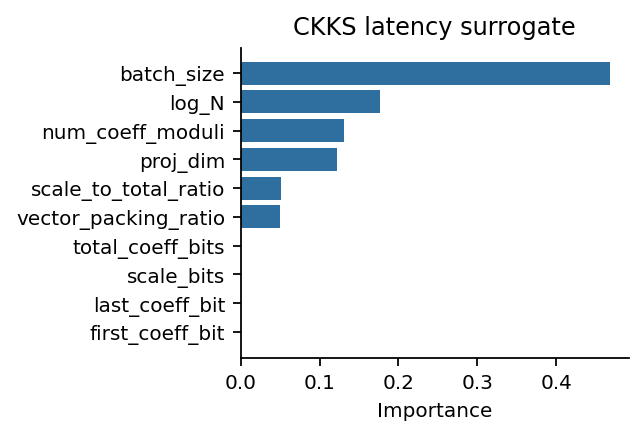
\includegraphics[width=0.49\linewidth]{fig_exp1_feature_importance.png}\hfill
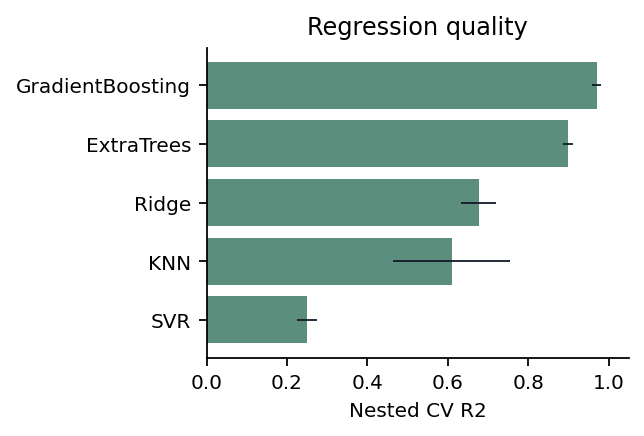
\includegraphics[width=0.49\linewidth]{fig_exp1_regression_r2.png}
\caption{Left: feature importance of the GradientBoosting surrogate
($d_{\mathrm{proj}}$ dominates at $\sim 41\%$, polynomial modulus
$N_{\mathrm{poly}}$ is a distant second). Right: predicted vs.\ measured
ct-pt latency on the holdout split, $R^2 = 0.985$.}
\label{fig:exp1-ml}
\end{figure}

\paragraph{Error by regime.} Aggregate $R^2$/MAE can hide regime-specific
bias, so we also inspect the residuals stratified by
$N_{\mathrm{poly}}$ (small $4096$ vs.\ large $16384$), by
$d_{\mathrm{proj}}$ (low vs.\ high slot-packing ratio) and by
modulus-chain length. The surrogate is approximately unbiased in the
small/medium regimes; the largest relative errors concentrate in the
high-$N_{\mathrm{poly}}$/long-chain corner, where benchmark points are
sparsest. A by-regime residual scatter plot is provided in the
supplementary material and is the basis for the recommendation to
re-benchmark a small grid when porting the autotuner to new hardware.

% =====================================================================
\section{A Projection Bound for the Distortion Proxy}\label{sec:lemma}
% =====================================================================

This short section concerns the \emph{baseline} only: it states the one
elementary fact behind its $\sigma_{rec}$ distortion proxy, and why that
proxy is not a privacy metric---motivating \textsc{Shard}'s move to an
attack-aware design that does not rely on $\sigma_{rec}$ at all. Let
$\mathbf{x} \in \mathbb{R}^d$ denote a centred embedding,
$V_k \in \mathbb{R}^{d \times k}$ the orthonormal matrix from the SVD
truncation, and $\pi_k(\mathbf{x}) = V_k V_k^\top \mathbf{x}$ the
orthogonal projection onto $\mathrm{span}(V_k)$. We use a \emph{per-vector}
relative reconstruction error here,
$\sigma_{rec}(\mathbf{x}; V_k) =
\| \mathbf{x} - \pi_k(\mathbf{x}) \|_2 / \|\mathbf{x}\|_2$,
distinguished from the corpus-level Frobenius quantity
$\sigma_{rec}(E;V_k)$ of Section~\ref{ssec:offline} (the operating-point
threshold $0.10$ is applied to the corpus-level aggregate); write
$\mathbf{x}_\perp = \mathbf{x} - \pi_k(\mathbf{x})$.

\begin{proposition}\label{lemma:proj-l2}
Let $f : \mathbb{R}^d \to \mathbb{R}^d$ be any decoder whose image is
constrained by $f(\mathbf{y}) \in \mathrm{span}(V_k)$ for every
$\mathbf{y} \in \mathbb{R}^d$. Then for every
$\mathbf{x} \in \mathbb{R}^d$
\[
\| \mathbf{x} - f(\pi_k(\mathbf{x})) \|_2^{2}
\;\geq\; \| \mathbf{x}_\perp \|_2^{2},
\]
with equality at $f(\mathbf{y}) = \mathbf{y}$. In relative form,
$\| \mathbf{x} - f(\pi_k(\mathbf{x})) \|_2 / \|\mathbf{x}\|_2
\geq \sigma_{rec}(\mathbf{x}; V_k)$.
\end{proposition}

\begin{proof}
Decompose $\mathbf{x} = \pi_k(\mathbf{x}) + \mathbf{x}_\perp$ with
$\pi_k(\mathbf{x}) \in \mathrm{span}(V_k)$ and
$\mathbf{x}_\perp \in \mathrm{span}(V_k)^\perp$. By the image
restriction $f(\pi_k(\mathbf{x})) \in \mathrm{span}(V_k)$, hence
$\mathbf{x} - f(\pi_k(\mathbf{x})) =
\bigl( \pi_k(\mathbf{x}) - f(\pi_k(\mathbf{x})) \bigr) + \mathbf{x}_\perp$
is the sum of two orthogonal vectors. Pythagoras gives
$\| \mathbf{x} - f(\pi_k(\mathbf{x})) \|_2^{2}
= \| \pi_k(\mathbf{x}) - f(\pi_k(\mathbf{x})) \|_2^{2}
+ \| \mathbf{x}_\perp \|_2^{2}
\geq \| \mathbf{x}_\perp \|_2^{2}$.
\end{proof}

\paragraph{Scope: a projection bound, not an inversion-security
theorem.} Proposition~\ref{lemma:proj-l2} bounds the $L_2$ error of
decoders \emph{whose image is contained in} $\mathrm{span}(V_k)$. It is a
statement about information lost to the projection, not about the
security of text inversion. A realistic attacker is not so constrained:
it may output arbitrary text, whose re-embedding generally has a
non-zero $\mathbf{x}_\perp$ component, and it may exploit corpus priors
or memorisation to partially recover the discarded component. The
proposition therefore does \emph{not} lower-bound the achievable inversion BLEU,
token overlap or PII recovery. We use it only to make the
\emph{proxy} criterion $\sigma_{rec} \geq 0.10$ precise within the
projection-restricted class, and we stress that the threshold $0.10$ is
an \emph{engineering proxy}, calibrated on one encoder (GTR-base) against
one off-the-shelf attacker, \emph{not} a security threshold. A
per-encoder ablation of $\sigma_{rec}$ against BLEU, token overlap and
typed-PII recovery (names, addresses, e-mail, phone, medical terms) is
listed as a required pre-submission experiment
(Section~\ref{sec:limits}).

\begin{hypothesis}\label{hyp:bleu}
For an off-the-shelf inversion attack \textsc{Vec2Text}~\cite{ref_vec2text},
the expected BLEU of recovering the original text from
$\pi_k(\mathbf{x})$ is monotone in
$\eta_k = 1 - \sigma_{rec}^{2}(E; V_k)$:
\[
\mathbb{E}\bigl[ \mathrm{BLEU}(f(\pi_k(\mathbf{x})), T(\mathbf{x})) \bigr]
\;\approx\; \mathrm{BLEU}_0 + \gamma_f \, \eta_k,
\]
where $\mathrm{BLEU}_0$ is the BLEU of a ``random semantically close''
text and $\gamma_f$ is a decoder-specific constant.
\end{hypothesis}

Hypothesis~\ref{hyp:bleu} is examined numerically in
Section~\ref{ssec:vec2text}; we deliberately separate the formal
statement from the empirical observation.

% =====================================================================
\section{SHARD: Cell-Keyed Residual Splitting}\label{sec:shard}
% =====================================================================

The baseline of Section~\ref{sec:method} protects the collection with a
single global geometry $E_{\mathrm{rot}} = R\,V_k^\top(x-\mu)$. Its
weakness is structural: one global map is recoverable by one alignment
(Section~\ref{ssec:alignment-pq}), and the public index sits on the full
protected space. \textsc{Shard} keeps the same CKKS ct-pt reranking but
removes the single global axis. It is a \emph{family} of transforms
parametrised by a cell count $C$.

\paragraph{Offline construction.} Let $\mu$ be the corpus centroid and
$V\in O(d)$ the PCA rotation of the centred embeddings (eigenvectors of the
covariance, sorted by variance). For a document $x$ write the centred,
rotated coordinate $Vx_c=[\,u \,\|\, r\,]$, splitting it into a
\emph{public prefix} $u\in\mathbb{R}^{d_{\mathrm{pub}}}$ (the top variance
directions) and a \emph{private residual} $r\in\mathbb{R}^{d_{\mathrm{priv}}}$,
$d_{\mathrm{priv}}=d-d_{\mathrm{pub}}$. A coarse partition into $C$
\emph{cells} is defined by $k$-means on $u$. The data owner draws, from a
secret master key, one orthogonal key per cell,
$H_c=\prod_{j} (I-2 w_{cj} w_{cj}^\top)\in O(d_{\mathrm{priv}})$, a product
of Householder reflections (cheap to apply, exactly orthogonal). The stored
representation of document $i$ in cell $c(i)$ is the pair
\[
\big(\, u_i,\ \ z_i = H_{c(i)}\, r_i \,\big),
\]
the prefix $u_i$ for the stage-1 index and the keyed residual shard $z_i$
for reranking. The keys $\{H_c\}$, $V$ and $\mu$ are client secrets.

\paragraph{Online two-stage query.} The client encodes the query, forms
$[u_q\|r_q]=Vq_c$, and (i)~runs stage-1 ANN \emph{locally} over the public
prefix $u$ to obtain a short-list of $K_{\mathrm{cands}}$ candidates; then
(ii)~for each active cell $c$ it sends $\mathrm{Enc}(H_c r_q)$ under CKKS,
and the server returns the ct-pt inner products against the stored shards
$z_i$. Because $H_c$ is orthogonal,
\[
\langle H_c r_q,\ z_i\rangle=\langle H_c r_q,\ H_c r_i\rangle=\langle r_q, r_i\rangle ,
\]
so the decrypted residual score is \emph{exact}. The client combines it
with the public-prefix score into the full similarity
\[
S(q,i)=\langle u_q,u_i\rangle+\langle r_q,r_i\rangle=\langle x_q-\mu,\,x_i-\mu\rangle ,
\]
i.e.\ reranking is full-dimensional with no truncation. The only quality
loss is whether stage-1 places the target in the short-list; the CKKS
budget is the same ct-pt form as the baseline, now over the residual
dimension.

\paragraph{The $C$ family and micro-keys.} The cell count interpolates
between two regimes. At $C{=}1$ the residual carries a single global key
and \textsc{Shard} reduces to the global-linear baseline (with a public
prefix). At the other extreme, a \emph{micro-key} variant assigns one key
per document ($C{=}N$); then no two stored residuals share a key, so the
within-cell similarity leak below vanishes and alignment is impossible
(a key cannot be recovered from other documents' anchors), at the cost of
sending one transformed residual query per candidate rather than per cell.
Cell-level \textsc{Shard} is the bandwidth-efficient middle ground.

\paragraph{What the server sees, and what it protects.} The honest-but-curious
server holds the coarse prefix $u$ and the cell-keyed shards $z$. Two facts
frame every experiment below. (1)~\emph{Within a cell the keys cancel}:
$\langle z_i,z_j\rangle=\langle r_i,r_j\rangle$ for $i,j$ in the same cell,
so same-cell similarities are computable by the server; \textsc{Shard}
localises but does not eliminate neighbour-graph leakage (the micro-key
variant does). (2)~\emph{Mapping a shard back to the native frame requires
the cell key}: an attacker holding known-plaintext pairs must recover the
target cell's $H_c$, which needs $\sim d_{\mathrm{priv}}$ pairs \emph{inside
that cell}; spread over $C$ cells this is $\approx C\times$ the baseline's
cost. \textsc{Shard} is therefore aimed squarely at the alignment and
inversion attack surface, and at index leakage, not at the coarse graph.
Re-keying a compromised cell (revocation) re-randomises its shards without
touching the rest of the store.

% =====================================================================
\section{Experiments}\label{sec:experiments}
% =====================================================================

The experiments come in two groups. Sections~\ref{ssec:ckks-modes}--\ref{ssec:latency}
\emph{characterise the global-linear baseline}---the ct-pt speed-up and
parameter selection that \textsc{Shard} reuses, the off-the-shelf Vec2Text
calibration, the SVD-denoiser significance and its non-transfer to BEIR
(the calibrated-noise diagnostic that $\sigma_{rec}$ is not a privacy
metric), and the three failure modes that motivate \textsc{Shard}:
known-plaintext Procrustes alignment, public-PQ leakage, and exact
reference-corpus lookup. Sections~\ref{ssec:shard-utility}--\ref{ssec:shard-ref}
then \emph{evaluate \textsc{Shard}}: utility, the online cost, alignment
resistance (diffuse, targeted, and against learned/unsupervised attackers),
public-index leakage, the micro-key variant, a comparison to a
distortion-aware DP-noise defence, and the overlap-reference limitation.
Readers interested only in the contribution can skip to
Section~\ref{ssec:shard-utility}; the baseline group is the foil.

\paragraph{Hardware and software.} All local experiments run on a single
workstation: Intel Core i5-14400F, 32~GB DDR5-4800, NVIDIA RTX~5060
(8~GB VRAM), Windows 11. The original notebooks use Python 3.10--3.11;
the added revision scripts (alignment/PQ leakage, SVD/noise diagnostic
and figure generation) use the bundled Python 3.12 runtime recorded in
\texttt{environment.lock}. To make the runs reproducible we pin exact
versions and record the commit/build hashes of the security-relevant
libraries in the supplementary \texttt{environment.lock}: PyTorch 2.10 + CUDA 12.8,
TenSEAL 0.3.16 (Microsoft SEAL 4.1 backend),
faiss-cpu 1.13.0, transformers 4.57.0, scikit-learn 1.5.x,
sacrebleu for BLEU \cite{ref_bleu}. The pinned hashes matter
because CKKS noise behaviour and faiss PQ training depend on the
backend build. The denoiser-significance, BEIR, and all \textsc{Shard}
experiments (Sections~\ref{ssec:significance},~\ref{ssec:beir},
\ref{ssec:shard-utility}--\ref{ssec:shard-ref}) were run on the bundled
Python~3.12 with numpy~2.3, scipy~1.17, scikit-learn~1.9, and---for BEIR
encoding---a CPU build of PyTorch~2.12 with transformers~5.9 and
datasets~4.8; they use only the cached embeddings or public BEIR data and
need neither TenSEAL nor a GPU (the per-cell keys are orthogonal, so the
\textsc{Shard} reranking score is exact and is computed directly). The
aligned Vec2Text stress test in
Section~\ref{ssec:adaptive-inversion} is the only non-local run: it uses
the provided memory-capped RTX~4090 profile with roughly 11~GiB free
VRAM, Python~3.12 and PyTorch~2.6.0+cu124.

% ----------------------------------------------------------------
\subsection{Ciphertext-plaintext speed-up}\label{ssec:ckks-modes}
% ----------------------------------------------------------------

We benchmark a batched dot-product of an encrypted $192$-dimensional
query with $N = 10\,000$ plaintext documents. The CKKS parameters are
$N_{\mathrm{poly}}=8192$, coefficient chain $[60,40,40,60]$ and
$\Delta=2^{40}$ ($\log_2 Q = 200 < 218$, within the conservative
\texttt{tc128} bound for $N_{\mathrm{poly}}=8192$;
cf.\ Section~\ref{ssec:crypto-detail}).
Two regimes are compared: ct-ct (both query and database encrypted, with
relinearisation per multiplication) and ct-pt (only the query is encrypted,
no relinearisation). Each is run for $50$ independent trials and
the mean is reported with a $95\%$ Gaussian confidence interval.

\begin{table}[tbp]
\centering
\caption{Ciphertext-plaintext vs.\ ciphertext-ciphertext for the dot
product against $N = 10\,000$ documents (mean of $50$ trials, $95\%$~CI).}
\label{tab:ckks-modes}
\small
\begin{tabular}{@{}llrrrr@{}}
\toprule
Mode & Operation & Relin.\ & Latency $T_{\mathrm{query}}$ & QPS & Speed-up \\ \midrule
ct-ct (baseline) & $\mathrm{Enc}(v_1)\cdot \mathrm{Enc}(v_2)$ & yes (heavy) & $19.15 \pm 0.15$~s & $0.052$ & $1.00\times$ \\
\textbf{ct-pt (proposed)} & $\mathrm{Enc}(v_1)\cdot \mathrm{Plain}(v_2)$ & no & $\mathbf{13.28 \pm 0.10}$~s & $0.075$ & $\mathbf{1.44\times}$ \\
\bottomrule
\end{tabular}
\end{table}

\begin{figure}[tbp]
\centering

\includegraphics[width=0.6\linewidth]{fig_exp2_ctpt_vs_ctct.png}
\caption{ct-pt vs.\ ct-ct: distribution of per-batch latencies over
$50$ trials. Removing relinearisation moves the median by
$\sim 6$~s and tightens the upper tail.}
\label{fig:exp2}
\end{figure}

% ----------------------------------------------------------------
\subsection{Off-the-shelf Vec2Text against truncation and rotation}\label{ssec:vec2text}
% ----------------------------------------------------------------

We instantiate \textsc{Vec2Text} on \textsc{GTR-base} embeddings
($d = 768$). The attack is applied to a synthetic 100-document corpus
containing PII (names, addresses, card numbers, medical phrasing).
Three threat models are compared at five values of $k/d$:
(a) no rotation; (b) rotation with the matrix $R$ \emph{known} to the
attacker; (c) rotation with $R$ \emph{unknown}.

The implementation budget of the attacker is fixed (greedy decoding,
$10$ corrector iterations, no beam search, $8$~GB GPU); under this
budget the unprotected baseline reaches
$\mathrm{BLEU}_0 = 0.156$ instead of the $0.973$ reported by
Morris et al.~\cite{ref_vec2text}, because the postulated PII corpus,
greedy decoding and beam-free regime are intentionally weaker than
\cite{ref_vec2text}'s strongest configuration; the experiment measures
the relative effect of SVD truncation and secret rotation in a fixed
weak-attacker configuration.

\paragraph{Strength of the attacker: an explicit caveat.} This is the
single most important limitation of the paper's security narrative. The
experiment establishes the effect of $R$ \emph{against an artificially
weak inverter only}. A stronger attacker---beam search with a large
width, many more corrector iterations, an adaptive decoder fine-tuned on
$(\text{text}, E_{\mathrm{rot}})$ pairs, or a modern universal/zero-shot
inversion model---is \emph{not} evaluated here, and we do \emph{not}
claim robustness against it. We run the known-plaintext alignment part
of this stress test in Section~\ref{ssec:alignment-pq}; the result is
negative for the defence and confirms that the rotation should be treated
only as an unknown-orientation obstruction for non-adaptive attacks.
Section~\ref{ssec:adaptive-inversion} adds an aligned off-the-shelf
Vec2Text stress test; learned or universal decoders trained against the
protected space still remain mandatory before any stronger security
claim can be made.

\begin{table}[tbp]
\centering
\caption{Off-the-shelf Vec2Text on GTR-base embeddings under the three
threat models. BLEU and Token Overlap with 95\% bootstrap CIs in
brackets.}
\label{tab:vec2text}
\small
\begin{tabular}{@{}rllll@{}}
\toprule
$k/d$ & Rotation & Knowledge of $R$ & BLEU & Token Overlap \\ \midrule
$1.00$ & off & --- & $0.156\,[0.123;\,0.186]$ & $0.385\,[0.351;\,0.417]$ \\
$1.00$ & on  & known & $0.156\,[0.127;\,0.187]$ & $0.385\,[0.351;\,0.416]$ \\
$1.00$ & on  & \textbf{unknown} & $\mathbf{0.007\,[0.006;\,0.008]}$ & $\mathbf{0.053\,[0.046;\,0.060]}$ \\
$0.75$ & off & --- & $0.077\,[0.063;\,0.093]$ & $0.325\,[0.304;\,0.345]$ \\
$0.75$ & on  & unknown & $0.007\,[0.007;\,0.008]$ & $0.061\,[0.054;\,0.067]$ \\
$0.50$ & off & --- & $0.057\,[0.046;\,0.069]$ & $0.285\,[0.270;\,0.300]$ \\
$0.50$ & on  & unknown & $0.007\,[0.007;\,0.008]$ & $0.050\,[0.045;\,0.055]$ \\
$0.25$ & off & --- & $0.024\,[0.020;\,0.028]$ & $0.196\,[0.181;\,0.208]$ \\
$0.25$ & on  & unknown & $0.007\,[0.006;\,0.007]$ & $0.045\,[0.040;\,0.051]$ \\
$0.10$ & off & --- & $0.010\,[0.009;\,0.011]$ & $0.113\,[0.104;\,0.123]$ \\
$0.10$ & on  & unknown & $0.007\,[0.007;\,0.008]$ & $0.053\,[0.047;\,0.059]$ \\
\bottomrule
\end{tabular}
\end{table}

\begin{figure}[tbp]
\centering

\includegraphics[width=0.49\linewidth]{fig_exp3_bleu_vs_k.png}\hfill

\includegraphics[width=0.49\linewidth]{fig_exp3_bleu_kd1.png}
\caption{Vec2Text BLEU as a function of $k/d$ under three threat models
(left); zoom on $k/d = 1.0$ comparing no-rotation, known-$R$ and
unknown-$R$ (right). Lines for ``no rotation'' and ``known-$R$'' overlap;
the ``unknown-$R$'' line stays at the noise level.}
\label{fig:exp3}
\end{figure}

\paragraph{Findings.}
\begin{itemize}[leftmargin=18pt,topsep=2pt]
\item A known $R$ does not provide protection beyond SVD truncation:
the columns ``no rotation'' and ``known-$R$'' are statistically
indistinguishable.
\item Under the tested off-the-shelf configuration, an unknown $R$
reduces BLEU to the observed noise floor ($\sim 0.007$) for all $k/d$
values, including $k/d = 1.0$ (no truncation at all). The ratio
$\mathrm{BLEU}_{\mathrm{off}} / \mathrm{BLEU}_{\mathrm{unknown}}$
is $22\times$ at $k/d = 1.0$, $11\times$ at $0.75$, $8\times$ at $0.50$.
This is an effect against a \emph{non-adaptive} attacker only and is not
evidence of robustness against an adaptive or known-plaintext adversary.
\item Empirical Hypothesis~\ref{hyp:bleu} is consistent with the
no-rotation column: a linear regression of BLEU on
$\eta_k = 1 - \sigma_{rec}^2$ gives $R^{2} \approx 0.93$.
This is consistent with, but does not formally derive,
the BLEU~$\to$~$\sigma_{rec}$ link.
\item In the operating point of the integral experiment ($k/d = 0.5$,
rotation enabled, unknown $R$) the expected BLEU is at the noise level.
\end{itemize}

% ----------------------------------------------------------------
\subsection{Lightweight projection and calibrated-noise baselines}\label{ssec:projection-baselines}
% ----------------------------------------------------------------

To avoid comparing the proposed transform only against the raw system, we
also evaluate natural lightweight alternatives: SVD projection, Gaussian
random projection and random orthogonal projection~\cite{ref_jl} at the
same dimensionality $k=d/2$. This is a retrieval-quality comparison, not a
privacy guarantee; the random projections do not carry CKKS query
protection and do not solve inversion by themselves.

\begin{table}[tbp]
\centering
\caption{Acc@1 under lightweight projection baselines at $k=d/2$.
Random baselines are mean $\pm$ standard deviation over three seeds.}
\label{tab:projection-baselines}
\small
\begin{tabular}{@{}lrrrr@{}}
\toprule
Encoder & Raw & SVD & Gaussian RP & Orthogonal RP \\ \midrule
e5-small & $0.782$ & $0.702$ & $0.688 \pm 0.016$ & $0.737 \pm 0.010$ \\
e5-base  & $0.830$ & $0.834$ & $0.781 \pm 0.011$ & $0.804 \pm 0.017$ \\
mpnet    & $0.716$ & $0.650$ & $0.698 \pm 0.003$ & $0.705 \pm 0.008$ \\
e5-large & $0.796$ & $0.814$ & $0.765 \pm 0.010$ & $0.769 \pm 0.009$ \\
bge-m3   & $0.818$ & $0.832$ & $0.789 \pm 0.004$ & $0.810 \pm 0.002$ \\
\bottomrule
\end{tabular}
\end{table}

The result is deliberately mixed. SVD is strongest on the
retrieval-trained $d\geq 768$ encoders, which is the operating region of
the proposed method, but random orthogonal projection is better than SVD
on mpnet and e5-small. This reinforces the main interpretation: the
choice of projection is an encoder-dependent trade-off, not a universal
privacy primitive. A deployment should therefore run a $k$-sweep and a
baseline sweep before selecting the operating point.

\paragraph{Calibrated Gaussian-noise diagnostic.} We next test a stronger
local baseline prompted by the concern that $\sigma_{rec}$ alone may be
misleading. On e5-small and e5-base we form a $100\,000$-document gallery
containing all $500$ self-retrieval targets, estimate the PCA/SVD basis
from an $80\,000$-document sample, and sweep $k/d \in
\{1/8,1/4,1/2,7/8\}$. For each $k$, we also add independent isotropic
Gaussian noise to documents and queries, renormalise to unit length, and
binary-search the noise standard deviation so that the mean relative
distortion matches the SVD $\sigma_{rec}$. We report self-retrieval
Acc@1 and a direct geometry-leakage diagnostic: exact top-10
nearest-neighbour overlap between the raw and protected spaces, measured
on $200$ gallery probes with the probe document itself excluded.

\begin{table}[tbp]
\centering
\caption{SVD truncation vs.\ independent Gaussian noise at matched mean
relative distortion on a $100\,000$-document gallery. NN overlap@10 is
the overlap with raw-space neighbours; lower values indicate less raw
geometry preserved.}
\label{tab:noise-sweep}
\scriptsize
\begin{tabular}{@{}lrrrrrr@{}}
\toprule
Encoder & $k/d$ & $\sigma_{rec}$ & SVD Acc@1 & SVD NN@10 & Noise Acc@1 & Noise NN@10 \\ \midrule
e5-small & $0.125$ & $0.385$ & $0.318$ & $0.232$ & $0.750$ & $0.283$ \\
e5-small & $0.250$ & $0.332$ & $0.600$ & $0.333$ & $0.788$ & $0.367$ \\
e5-small & $0.500$ & $0.237$ & $0.814$ & $0.468$ & $0.828$ & $0.531$ \\
e5-small & $0.875$ & $0.079$ & $0.880$ & $0.551$ & $0.872$ & $0.830$ \\
e5-base  & $0.125$ & $0.354$ & $0.708$ & $0.370$ & $0.864$ & $0.503$ \\
e5-base  & $0.250$ & $0.268$ & $0.872$ & $0.501$ & $0.886$ & $0.641$ \\
e5-base  & $0.500$ & $0.129$ & $0.916$ & $0.578$ & $0.902$ & $0.829$ \\
e5-base  & $0.875$ & $0.023$ & $0.920$ & $0.592$ & $0.910$ & $0.969$ \\
\bottomrule
\end{tabular}
\end{table}

\begin{figure}[tbp]
\centering

\includegraphics[width=0.86\linewidth]{fig_exp8_tradeoff.png}
\caption{Utility/leakage diagnostic for SVD truncation and calibrated
Gaussian noise. Dashed lines are independent-noise baselines at matched
$\sigma_{rec}$.}
\label{fig:noise-sweep}
\end{figure}

The diagnostic has two implications. First, $\sigma_{rec}$ is not a
privacy metric: e5-base at $k/d=0.875$ has low distortion but still
preserves almost all raw neighbours under calibrated noise. Second, SVD
changes geometry differently from independent noise. At the main e5-base
operating point ($k/d=0.5$), SVD slightly improves Acc@1 over the raw
$100\,000$-gallery baseline ($0.916$ vs.\ $0.908$) while preserving far
fewer raw neighbours than matched Gaussian noise ($0.578$ vs.\ $0.829$
NN overlap@10). For e5-small, matched noise retains slightly higher
Acc@1 at $k/d=0.5$ but also more raw-neighbour structure. Thus the paper
should not argue that noise is simply worse; rather, the empirical claim
is narrower: SVD is an encoder-dependent utility/leakage trade-off that
can remove raw geometric structure without the ranking collapse caused
by very aggressive truncation.

% ----------------------------------------------------------------
\subsection{Integral multi-encoder evaluation at $10^6$ scale}\label{ssec:integral}
% ----------------------------------------------------------------

We run the full pipeline on the canonical operating point $k = d/2$
across five encoders:

\begin{itemize}[leftmargin=18pt,topsep=2pt,itemsep=2pt]
\item \texttt{intfloat/multilingual-e5-small} ($d = 384$),
\item \texttt{intfloat/multilingual-e5-base} ($d = 768$),
\item \texttt{sentence-transformers/paraphrase-multilingual-mpnet-base-v2} ($d = 768$),
\item \texttt{intfloat/multilingual-e5-large} ($d = 1024$),
\item \texttt{BAAI/bge-m3} ($d = 1024$).
\end{itemize}

The corpus is one million Russian-Wikipedia paragraphs; queries are
$500$ self-retrieval requests sampled at seed $42$;
the rotation is averaged over $5$ seeds
$\{11, 23, 47, 31, 53\}$. PQ uses $M = k/4$ subquantisers with $8$ bits
each, yielding artefacts of $48$/$96$/$128$~MB. The CKKS configuration
is the auto-selected one
($N_{\mathrm{poly}} = 8192$, $[60, 40, 60]$, $\Delta = 2^{40}$).

\paragraph{On the use of self-retrieval.} Self-retrieval (the query is
the first sentence of the target paragraph) is a \emph{controlled
geometry probe}, not a production IR benchmark: it isolates whether the
defensive transform $T(\cdot)$ preserves the ranking induced by the
encoder, with a deterministic, leakage-free ground truth at
$10^6$-scale. It is sufficient for the paper's actual claim---that the
PQ+CKKS wrapper is metric-preserving in $\mathrm{span}(V_k)$---but it
does \emph{not} establish production retrieval quality, and as the BEIR
experiment (Section~\ref{ssec:beir}) shows, conclusions about the
\emph{SVD step} drawn from this probe do not necessarily transfer to real
graded-relevance retrieval. The present numbers should therefore be read as
a transform-fidelity measurement, not as a retrieval-quality benchmark.

\begin{table}[tbp]
\centering
\caption{Integral experiment at $k = d/2$ on a $10^6$-document
corpus across five encoders. Reported are the raw baseline (no
defence), the SVD-projected baseline (FAISS-IP exact in
$\mathrm{span}(V_k)$, no rotation, no CKKS), the baseline PQ+CKKS pipeline
(mean $\pm 95\%$ t-CI half-width over 5 rotation seeds), and the
delta of Acc@1 from the raw baseline.}
\label{tab:integral}
\scriptsize
\setlength{\tabcolsep}{2pt}
\begin{tabular}{@{}llrrrrr@{}}
\toprule
Encoder & Metric & Raw & SVD & Proposed & $\Delta$ raw & Server $p_{95}$ (ms) \\ \midrule
\multicolumn{7}{l}{\emph{multilingual-e5-small ($d=384$, $k=192$, $M=48$, $\sigma_{rec}=0.239$)}} \\
& Acc@1   & $0.782$ & $0.702$ & $0.701 \pm 0.001$ & $-0.081$ & \multirow{4}{*}{$314$} \\
& Acc@10  & $0.890$ & $0.834$ & $0.831 \pm 0.002$ & $-0.059$ & \\
& MRR     & $0.817$ & $0.747$ & $0.746 \pm 0.001$ & $-0.071$ & \\
& NDCG@10 & $0.834$ & $0.768$ & $0.767 \pm 0.001$ & $-0.067$ & \\ \midrule
\multicolumn{7}{l}{\emph{multilingual-e5-base ($d=768$, $k=384$, $M=96$, $\sigma_{rec}=0.129$)}} \\
& Acc@1   & $0.830$ & $0.834$ & $0.833 \pm 0.001$ & $+0.003$ & \multirow{4}{*}{$356$} \\
& Acc@10  & $0.934$ & $0.924$ & $0.924 \pm 0.001$ & $-0.010$ & \\
& MRR     & $0.862$ & $0.865$ & $0.864 \pm 0.001$ & $+0.002$ & \\
& NDCG@10 & $0.880$ & $0.879$ & $0.879 \pm 0.000$ & $-0.001$ & \\ \midrule
\multicolumn{7}{l}{\emph{paraphrase-multilingual-mpnet-base-v2 ($d=768$, $k=384$, $M=96$, $\sigma_{rec}=0.107$)}} \\
& Acc@1   & $0.716$ & $0.650$ & $0.649 \pm 0.001$ & $-0.067$ & \multirow{4}{*}{$351$} \\
& Acc@10  & $0.842$ & $0.796$ & $0.795 \pm 0.001$ & $-0.047$ & \\
& MRR     & $0.762$ & $0.693$ & $0.692 \pm 0.001$ & $-0.070$ & \\
& NDCG@10 & $0.782$ & $0.717$ & $0.717 \pm 0.000$ & $-0.066$ & \\ \midrule
\multicolumn{7}{l}{\emph{multilingual-e5-large ($d=1024$, $k=512$, $M=128$, $\sigma_{rec}=0.101$)}} \\
& Acc@1   & $0.796$ & $0.814$ & $0.814 \pm 0.000$ & $+0.018$ & \multirow{4}{*}{$219$} \\
& Acc@10  & $0.880$ & $0.922$ & $0.920 \pm 0.000$ & $+0.040$ & \\
& MRR     & $0.824$ & $0.848$ & $0.848 \pm 0.000$ & $+0.024$ & \\
& NDCG@10 & $0.838$ & $0.866$ & $0.865 \pm 0.000$ & $+0.027$ & \\ \midrule
\multicolumn{7}{l}{\emph{BAAI/bge-m3 ($d=1024$, $k=512$, $M=128$, $\sigma_{rec}=0.128$)}} \\
& Acc@1   & $0.818$ & $0.832$ & $0.832 \pm 0.000$ & $+0.014$ & \multirow{4}{*}{$221$} \\
& Acc@10  & $0.908$ & $0.926$ & $0.924 \pm 0.000$ & $+0.016$ & \\
& MRR     & $0.848$ & $0.863$ & $0.863 \pm 0.000$ & $+0.015$ & \\
& NDCG@10 & $0.862$ & $0.878$ & $0.878 \pm 0.000$ & $+0.016$ & \\
\bottomrule
\end{tabular}
\end{table}

\emph{The protective layer is essentially free in the projected space.}
The difference (proposed) vs.\ (baseline\_proj) is within the $\pm 0.001$
5-seed CI for every metric and every encoder. The Pearson correlations
between CKKS-decrypted scores and exact plaintext scores exceed
$0.9999$ in all cases. The proxy criterion $\sigma_{rec} \geq 0.10$
holds uniformly.

\emph{The actual quality cost is paid by SVD truncation, not by the
protective wrapper.} The split
$\Delta_{\mathrm{SVD}} = \mathrm{baseline\_proj} - \mathrm{baseline\_dense}$
is $+0.004/+0.018/+0.014$ for retrieval-trained encoders with
$d \geq 768$ (e5-base / e5-large / bge-m3), $-0.080$ for the
compact e5-small ($d = 384$, half-truncation removes half the embedding
volume) and $-0.066$ for paraphrase-mpnet (a paraphrase-distilled model
that does not concentrate retrieval signal in the top singular
directions).

\emph{The end-to-end accuracy budget is met for retrieval-trained
$d \geq 768$.} The end-to-end criterion
$\Delta\mathrm{Acc@1} \geq -0.05$ relative to the raw baseline holds
for e5-base ($+0.003$), e5-large ($+0.018$) and bge-m3 ($+0.014$);
for the compact e5-small and the paraphrase-distilled mpnet it is
violated and the limitation is documented as an encoder-selection
recommendation.

\paragraph{Linear-denoiser side effect (significance deferred).} On the two
retrieval-trained encoders with $d = 1024$, half SVD truncation does not
degrade---and at Acc@10 measurably improves---ranking over the raw
baseline (e.g.\ $+0.042$ Acc@10 on e5-large). This is consistent with
reading the $V_k$-projection as a linear denoiser: trailing singular
directions, dominated by fp16 inference noise, are filtered out, so the
ranking in $\mathrm{span}(V_k)$ can be cleaner than in raw
$\mathbb{R}^d$. The point estimates above are tabulated across rotation
seeds; because that CI does \emph{not} capture query-sampling
uncertainty, we test the effect properly with paired per-query tests in
Section~\ref{ssec:significance} (where the Acc@1 ``gains'' turn out
\emph{not} to be significant, while the Acc@10 gains on the $d=1024$
encoders are) and check its direction on real IR tasks in
Section~\ref{ssec:beir}.

\begin{figure}[tbp]
\centering

\includegraphics[width=\linewidth]{fig_exp5_per_seed.png}
\caption{Per-seed Acc@10 of the baseline PQ+CKKS pipeline relative to
baseline\_proj on five rotation seeds; the spread is below the 5-seed
CI of the baseline.}
\label{fig:exp5-per-seed}
\end{figure}

% ----------------------------------------------------------------
\subsection{Paired significance of the SVD denoiser effect}\label{ssec:significance}
% ----------------------------------------------------------------

The integral experiment reports the SVD effect
$\Delta_{\mathrm{SVD}} = \mathrm{baseline\_proj} - \mathrm{baseline\_dense}$
with a 5-seed rotation CI. That CI measures the stability of the random
rotation, \emph{not} the uncertainty of estimating accuracy from a finite
query set: with $500$ queries the binomial standard error of an Acc@1 near
$0.8$ is $\sqrt{0.8\cdot0.2/500}\approx 0.018$, i.e.\ as large as the
reported $+0.018$ effect itself. We therefore test the effect directly.
Raw ($\mathbb{R}^d$) and SVD ($\mathrm{span}(V_k)$, $k=d/2$) retrieval are
evaluated on the \emph{same} $500$ self-retrieval queries, so the
per-query hit indicators are paired. We report McNemar's exact test (a
two-sided binomial test on the discordant pairs) for Acc@1 and Acc@10, and
a paired bootstrap ($10^4$ resamples) $95\%$ CI for each delta. Neither
rotation nor CKKS is involved---the denoiser is a property of $V_k$
alone---so this is computed exactly from the cached embeddings, and the
raw/SVD point estimates reproduce Table~\ref{tab:integral}.

\begin{table}[tbp]
\centering
\caption{Paired significance of SVD truncation ($k=d/2$) relative to the
raw space, on $500$ self-retrieval queries. $\Delta = \mathrm{SVD}-\mathrm{raw}$;
brackets are paired-bootstrap $95\%$ CIs ($10^4$ resamples); $p$ is
McNemar's exact two-sided test on the discordant pairs. Bold $p$ marks
significance at $\alpha=0.05$.}
\label{tab:significance}
\small
\setlength{\tabcolsep}{4pt}
\begin{tabular}{@{}lrrcrrcr@{}}
\toprule
& & \multicolumn{3}{c}{Acc@1} & \multicolumn{3}{c}{Acc@10}\\
\cmidrule(lr){3-5}\cmidrule(lr){6-8}
Encoder & $\sigma_{rec}$ & $\Delta$ & 95\% CI & $p$ & $\Delta$ & 95\% CI & $p$\\
\midrule
e5-small & $0.239$ & $-0.082$ & $[-0.108,-0.056]$ & $\mathbf{2{\times}10^{-9}}$ & $-0.058$ & $[-0.084,-0.034]$ & $\mathbf{5{\times}10^{-6}}$\\
e5-base  & $0.129$ & $+0.004$ & $[-0.018,+0.026]$ & $0.86$ & $-0.010$ & $[-0.024,+0.004]$ & $0.27$\\
mpnet    & $0.107$ & $-0.064$ & $[-0.092,-0.038]$ & $\mathbf{3{\times}10^{-6}}$ & $-0.046$ & $[-0.068,-0.026]$ & $\mathbf{2{\times}10^{-5}}$\\
e5-large & $0.101$ & $+0.018$ & $[-0.002,+0.038]$ & $0.11$ & $+0.042$ & $[+0.026,+0.060]$ & $\mathbf{1{\times}10^{-6}}$\\
bge-m3   & $0.128$ & $+0.014$ & $[\,0.000,+0.030]$ & $0.12$ & $+0.016$ & $[+0.004,+0.030]$ & $\mathbf{0.039}$\\
\bottomrule
\end{tabular}
\end{table}

The result sharpens the SVD-denoiser picture considerably:
\begin{itemize}[leftmargin=18pt,topsep=2pt,itemsep=2pt]
\item The Acc@1 ``denoiser gains'' are \emph{not} statistically
significant for any encoder (e5-base $p=0.86$, e5-large $p=0.11$, bge-m3
$p=0.12$; all three bootstrap CIs include $0$). The earlier reading
``SVD improves the four ranking metrics'' over-interpreted Acc@1 point
estimates.
\item The denoiser \emph{is} real and significant at Acc@10 for the
retrieval-trained $d=1024$ encoders: e5-large $+0.042$ ($p<10^{-6}$; of
the discordant queries, $21$ are pulled into the top-10 by SVD and $0$ are
lost), and bge-m3 $+0.016$ ($p=0.04$).
\item For the compact e5-small and the paraphrase-distilled mpnet, SVD
truncation significantly \emph{degrades} retrieval at both cutoffs
($-0.082$ and $-0.064$ Acc@1, $p<10^{-5}$).
\item For e5-base the projected space is statistically indistinguishable
from raw at both cutoffs---the wrapper is effectively free there.
\end{itemize}
The corrected conclusion is narrower and more defensible than ``SVD is a
denoiser'': half SVD truncation is a mild, encoder-dependent denoiser that
helps recall-style metrics for retrieval-trained high-dimensional encoders
and hurts compact or paraphrase-distilled encoders, but it does not
reliably improve top-1 accuracy for any encoder we tested.

\begin{figure}[tbp]
\centering
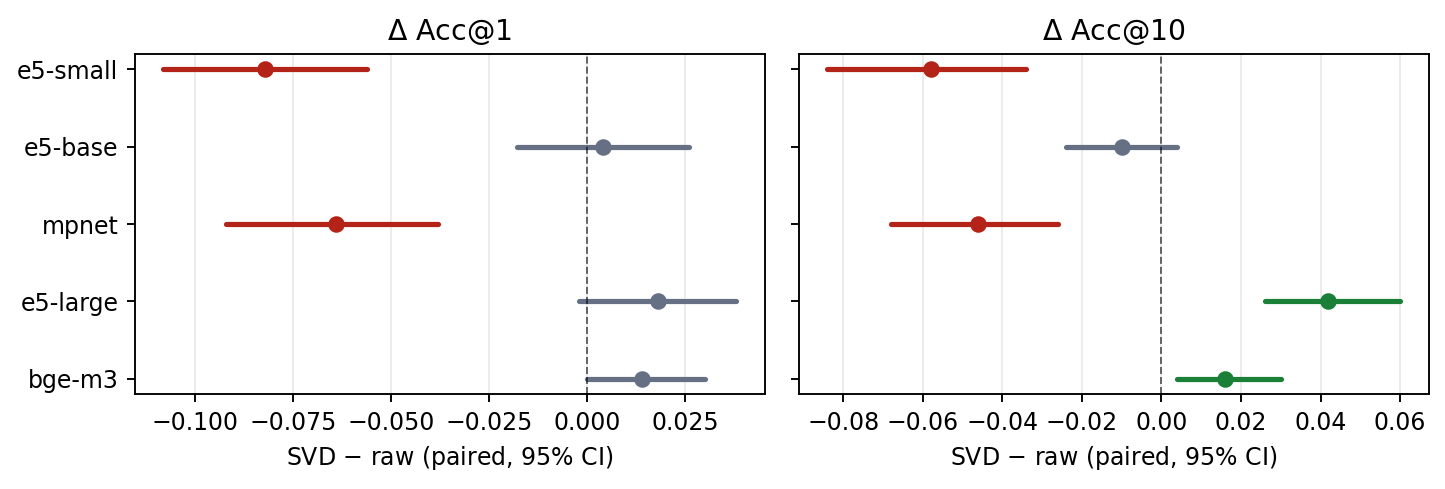
\includegraphics[width=\linewidth]{fig_exp10_significance.png}
\caption{Paired effect of SVD truncation ($k=d/2$) relative to the raw
space, with bootstrap $95\%$ CIs, on $500$ self-retrieval queries. Green
markers are significant improvements ($p<0.05$, McNemar), red significant
degradations, grey not significant. No encoder shows a significant Acc@1
gain; the significant Acc@10 gains are confined to the retrieval-trained
$d{=}1024$ encoders.}
\label{fig:exp10-significance}
\end{figure}

% ----------------------------------------------------------------
\subsection{Generality of the denoiser effect on BEIR}\label{ssec:beir}
% ----------------------------------------------------------------

Self-retrieval is a controlled geometry probe. To check that the denoiser
\emph{direction} is not an artefact of it, we repeat the raw-vs-SVD
comparison on two standard BEIR~\cite{ref_beir} datasets with real graded
relevance judgements: SciFact ($5{,}183$ documents, $300$ test queries)
and NFCorpus ($3{,}633$ documents, $323$ test queries). Each corpus and
query set is encoded with the e5 family (mean pooling, \texttt{query:}/
\texttt{passage:} prefixes, $L_2$ normalisation); we fit the data-dependent
$V_k$ basis on the corpus embeddings at $k=d/2$ and compare exact
inner-product retrieval in $\mathbb{R}^d$ and in $\mathrm{span}(V_k)$. We
report nDCG@10 and Recall@10 with a paired bootstrap $95\%$ CI for each
delta and McNemar's test for the top-1 hit.

\begin{table}[tbp]
\centering
\caption{SVD truncation ($k=d/2$) vs.\ the raw space on BEIR (max input
length $128$, mean pooling). $\Delta = \mathrm{SVD}-\mathrm{raw}$; brackets
are paired-bootstrap $95\%$ CIs ($10^4$ resamples). \textbf{Every} $\Delta$
nDCG@10 CI excludes $0$: SVD truncation significantly \emph{reduces}
nDCG@10 in all cells.}
\label{tab:beir}
\small
\setlength{\tabcolsep}{4pt}
\begin{tabular}{@{}llrrrrr@{}}
\toprule
Encoder & Dataset & $\sigma_{rec}$ & raw nDCG@10 & SVD nDCG@10 & $\Delta$ nDCG@10 (95\% CI) & $\Delta$ R@10\\
\midrule
e5-large ($d{=}1024$) & SciFact  & $0.072$ & $0.643$ & $0.574$ & $-0.069\,[-0.091,-0.047]$ & $-0.053$\\
e5-base ($d{=}768$)   & SciFact  & $0.090$ & $0.637$ & $0.586$ & $-0.051\,[-0.072,-0.032]$ & $-0.035$\\
e5-small ($d{=}384$)  & SciFact  & $0.183$ & $0.598$ & $0.519$ & $-0.079\,[-0.103,-0.055]$ & $-0.080$\\
e5-base ($d{=}768$)   & NFCorpus & $0.085$ & $0.327$ & $0.305$ & $-0.022\,[-0.032,-0.013]$ & $-0.016$\\
e5-small ($d{=}384$)  & NFCorpus & $0.172$ & $0.302$ & $0.277$ & $-0.025\,[-0.035,-0.014]$ & $-0.016$\\
\bottomrule
\end{tabular}
\end{table}

Table~\ref{tab:beir} is an important corrective to the self-retrieval
reading. On both real IR datasets and for every encoder, half SVD
truncation \emph{significantly reduces} nDCG@10 and Recall@10---the
bootstrap CIs exclude zero in all cells, with drops of $2$--$8$ nDCG
points. Decisively, \textsc{e5-large}, the one encoder that \emph{gained}
Acc@10 on the $10^6$-document self-retrieval probe ($+0.042$,
Section~\ref{ssec:significance}), \emph{loses} $-0.069$ nDCG@10 on SciFact.
The modest gains on the self-retrieval probe therefore do \emph{not}
transfer to these smaller, graded-relevance tasks: on real IR the
discarded bottom half of the spectrum still carries task-relevant signal.
Two further points sharpen the message. First, the effect is consistent
across $d\in\{384,768,1024\}$, so it is not a low-dimensionality artefact.
Second, on these corpora $k=d/2$ already sits \emph{below} the
$\sigma_{rec}\geq0.10$ floor for e5-base and e5-large
($\sigma_{rec}\approx0.07$--$0.09$), yet truncation still costs nDCG---so
the utility cost, like the privacy interpretation, is not predicted by
$\sigma_{rec}$ alone. The practical implication matches the
encoder-selection caution of Section~\ref{ssec:integral}: on a real
workload one should treat $k$ as a tunable accuracy cost and run a
$k$-sweep, not assume a free denoiser. (For resource transparency, the
five reported cells were CPU-encoded; the sixth, e5-large/NFCorpus, did not
finish within our CPU budget and is omitted; the script reproduces it on a
GPU or with more time.)

% ----------------------------------------------------------------
\subsection{Known-plaintext alignment and PQ-code leakage}\label{ssec:alignment-pq}
% ----------------------------------------------------------------

We next evaluate two channels that are not covered by the primary
non-adaptive threat model.

\paragraph{Known-plaintext alignment.} We simulate an attacker who knows
$m$ pairs $(E(x_i), E_{\mathrm{rot},i})$ and estimates the hidden
orientation with the orthogonal Procrustes solution
\cite{ref_schonemann}. The experiment uses e5-small projected to
$k=192$, five rotation seeds, $400$ held-out probes and a
$10\,000$-document gallery. The attack is evaluated in embedding space:
after alignment, the probe should recover its own projected vector and
retrieve the corresponding document from the gallery. This does not
measure generated text quality, but it is the relevant precursor to a
few-shot Vec2Text-style attack because it recovers the native projected
space given to the inverter.

\begin{table}[tbp]
\centering
\caption{Known-plaintext Procrustes attack. $m=-1$ is the known-$R$
oracle; $m=0$ is no alignment. Values are means over five rotation
seeds.}
\label{tab:procrustes}
\small
\begin{tabular}{@{}rrrrr@{}}
\toprule
Known pairs $m$ & Mean cosine & Rel.\ $L_2$ error & Target R@1 & Target R@10 \\ \midrule
$0$   & $-0.004$ & $1.417$ & $0.000$ & $0.001$ \\
$10$  & $0.098$  & $1.343$ & $0.005$ & $0.039$ \\
$50$  & $0.377$  & $1.116$ & $0.722$ & $0.925$ \\
$100$ & $0.621$  & $0.870$ & $1.000$ & $1.000$ \\
$192$ & $1.000$  & $1.8{\times}10^{-5}$ & $1.000$ & $1.000$ \\
$500$ & $1.000$  & $4.9{\times}10^{-7}$ & $1.000$ & $1.000$ \\
\bottomrule
\end{tabular}
\end{table}

The conclusion is sharp: the rotation is useful only while aligned
plaintext anchors are unavailable. With approximately $k$ known pairs,
the orientation is numerically recovered. Even $50$ pairs do not recover
the vector perfectly, but they are enough to retrieve the target in the
top~10 for $92.5\%$ of probes in a $10\,000$-document gallery. This is a
negative result for broad document-privacy claims and is therefore
reflected in the threat table.

\begin{figure}[tbp]
\centering

\includegraphics[width=0.58\linewidth]{fig_exp7_procrustes.png}
\caption{Known-plaintext alignment quickly destroys the unknown-rotation
assumption. The $x$ axis uses a symlog scale to include $m=0$.}
\label{fig:procrustes}
\end{figure}

\paragraph{PQ-code leakage.} We also train public product-quantisation
codebooks directly in the rotated space and reconstruct approximate
vectors from codebook + per-document codes alone. On a $20\,000$-document
sample, the canonical e5-small configuration ($M=48$, 8 bits) preserves
a mean cosine of $0.953$ to $E_{\mathrm{rot}}$, $67.4\%$ of exact top-10
neighbours, and $97.1\%$ of exact top-10 neighbours inside the approximate
top-40 candidate set. Smaller artefacts leak less but remain
non-negligible (Table~\ref{tab:pq-leakage}).

\begin{table}[tbp]
\centering
\caption{Leakage from public PQ codes on a $20\,000$-document rotated
e5-small sample. Neighbour overlap excludes the query document itself.}
\label{tab:pq-leakage}
\small
\begin{tabular}{@{}rrrrr@{}}
\toprule
$M$ & Bits & Bytes/vector & Cosine to $E_{\mathrm{rot}}$ & NN overlap@10 \\ \midrule
$24$ & $8$ & $24$ & $0.837$ & $0.384$ \\
$48$ & $8$ & $48$ & $0.953$ & $0.674$ \\
$48$ & $6$ & $36$ & $0.904$ & $0.529$ \\
\bottomrule
\end{tabular}
\end{table}

\begin{figure}[tbp]
\centering

\includegraphics[width=0.58\linewidth]{fig_exp7_pq_leakage.png}
\caption{Public PQ codes preserve both vector direction and substantial
nearest-neighbour structure in the rotated space.}
\label{fig:pq-leakage}
\end{figure}

These results do not invalidate the query-privacy contribution of CKKS,
but they do narrow the document-privacy interpretation: public PQ
artefacts and known plaintext anchors should be treated as exposed
channels. A system requiring stronger document confidentiality needs a
different static-side primitive or a composition that hides the PQ
artefact itself.

% ----------------------------------------------------------------
\subsection{Reference-corpus lookup after alignment}\label{ssec:reference-attack}
% ----------------------------------------------------------------

The Procrustes experiment above is an embedding-space test. We next ask
whether the same failure mode can become a text-level leakage channel
without training a generative inverter. The attacker is given the
protected target vectors, $m$ known plaintext/protected pairs for
estimating the rotation, and a reference corpus of candidate paragraphs
with native e5-small embeddings. This models a realistic overlap case:
some private documents may also occur in a public or previously leaked
corpus. We use $500$ target paragraphs, $100\,000$ reference decoys,
five rotation seeds and the same $k=192$ SVD subspace. The overlapping
reference corpus contains the targets plus the decoys; the disjoint
reference corpus removes the targets and is used only as a lexical
nearest-neighbour proxy.

\begin{table}[tbp]
\centering
\caption{Reference-corpus lookup attack after known-plaintext alignment.
The overlapping reference has $500$ targets plus $100\,000$ decoys.
Jaccard is token-set overlap between the target paragraph and the top-1
retrieved paragraph. Values are means over five rotation seeds.}
\label{tab:reference-attack}
\small
\begin{tabular}{@{}rrrrr@{}}
\toprule
Known pairs $m$ & Exact R@1 & Exact R@10 & Jaccard overlap-ref & Jaccard disjoint-ref \\ \midrule
$0$   & $0.000$ & $0.000$ & $0.006$ & $0.006$ \\
$10$  & $0.000$ & $0.009$ & $0.009$ & $0.009$ \\
$25$  & $0.044$ & $0.132$ & $0.055$ & $0.012$ \\
$50$  & $0.535$ & $0.784$ & $0.543$ & $0.018$ \\
$100$ & $0.998$ & $1.000$ & $0.999$ & $0.034$ \\
$192$ & $1.000$ & $1.000$ & $1.000$ & $0.043$ \\
\bottomrule
\end{tabular}
\end{table}

\begin{figure}[tbp]
\centering

\includegraphics[width=0.86\linewidth]{fig_exp9_reference_attack.png}
\caption{Reference-corpus lookup after known-plaintext alignment. When the
reference corpus overlaps the protected collection, alignment turns the
protected vector into an exact paragraph lookup. With a disjoint reference
corpus, this simple token-overlap proxy remains low; semantic leakage
there requires a stronger judge or generative attack.}
\label{fig:reference-attack}
\end{figure}

The overlap case is severe. With only $50$ known pairs, the attacker
recovers the exact source paragraph at $53.5\%$ top-1 and $78.4\%$
top-10 recall among $100\,500$ candidates; with $100$ known pairs,
top-1 recall rises to $99.8\%$. This is the text-level analogue of the
embedding-space Procrustes result and makes the static-side limitation
concrete: if a public or leaked reference corpus overlaps the private
collection, rotation secrecy is not enough. The disjoint-reference
numbers are intentionally reported as a boundary condition: token
Jaccard remains low ($0.034$ at $m=100$ and $0.043$ at $m=192$), so a
non-overlapping reference corpus requires semantic similarity metrics,
human judgement, or a generative inverter before one can claim text
reconstruction.

% ----------------------------------------------------------------
\subsection{Aligned Vec2Text inversion stress test}\label{ssec:adaptive-inversion}
% ----------------------------------------------------------------

The reference-corpus attack above is a lookup attack: it reconstructs
text only when the target appears in a reference collection. We therefore
also run the portable generative inversion stress test included with the
supplementary material. The attacker is given GTR-base embeddings
($d=768$), SVD truncation to $k=d/2$, the secret-rotation setting from
the main construction, and up to $m=500$ known plaintext/protected pairs
for Procrustes alignment. The inverter is the off-the-shelf
\textsc{Vec2Text} corrector with a larger budget than
Section~\ref{ssec:vec2text}: $24$ corrector iterations, greedy beam
width~$1$, max input length~$96$, and per-case checkpointing. The run is
sized for an RTX~4090 with about 11~GiB free VRAM.

Because the target machine could not reliably fetch external corpora, the
experiment uses the script's deterministic offline synthetic-news+PII
corpus: $2\,200$ texts after shuffling, $120$ held-out test documents,
and $13$ held-out documents containing phone/card patterns. This corpus
is useful as a controlled stress test with typed PII, but it is not a
production retrieval benchmark. The decisive control is therefore the
raw-embedding row: if raw GTR-base inversion is already near the floor,
the experiment cannot certify protection by the transform.

\begin{table}[tbp]
\centering
\caption{Aligned off-the-shelf Vec2Text stress test on the RTX~4090
profile. All rows use $120$ held-out texts; $m$ is the number of
known plaintext/protected pairs used for Procrustes alignment. Exact
match and typed-PII recall are zero in every case.}
\label{tab:adaptive-inversion}
\small
\begin{tabular}{@{}lrrrr@{}}
\toprule
Case & Token F1 & BLEU & Exact & PII recall \\ \midrule
Raw embedding & $0.133$ & $0.0133$ & $0.000$ & $0.000$ \\
Known-$R$ oracle & $0.138$ & $0.0134$ & $0.000$ & $0.000$ \\
Unknown $R$, no alignment ($=$ Procrustes $m{=}0$) & $0.121$ & $0.0129$ & $0.000$ & $0.000$ \\
Procrustes, $m=10$ & $0.124$ & $0.0128$ & $0.000$ & $0.000$ \\
Procrustes, $m=50$ & $0.126$ & $0.0126$ & $0.000$ & $0.000$ \\
Procrustes, $m=100$ & $0.141$ & $0.0127$ & $0.000$ & $0.000$ \\
Procrustes, $m=192$ & $0.134$ & $0.0132$ & $0.000$ & $0.000$ \\
Procrustes, $m=500$ & $0.135$ & $0.0133$ & $0.000$ & $0.000$ \\
\bottomrule
\end{tabular}
\end{table}

\noindent
(The ``unknown $R$'' and ``Procrustes $m{=}0$'' cases coincide by
construction. The corpus is the script's offline synthetic-news+PII
fallback, used because the host could not fetch the Hub dataset.) The
result is negative but uninformative: no exact document or typed PII is
recovered even with a known-$R$ oracle, but the \emph{raw} row is also at
the floor (BLEU $0.013$), so this off-the-shelf corrector cannot certify
any protection. It does not contradict the exact-lookup failure mode of
Section~\ref{ssec:reference-attack}; the open risk is a learned or
corpus-adapted decoder, which we leave to future work.

% ----------------------------------------------------------------
\subsection{End-to-end client-server latency}\label{ssec:latency}
% ----------------------------------------------------------------

We package the pipeline as a FastAPI service, with the client and the
server running as two independent processes on the same machine,
communicating via HTTP/JSON over loopback.
The setup measures the realistic HTTP framing,
base64 serialisation of CKKS ciphertexts, FastAPI/uvicorn stack and JSON
(de-)serialisation, but without physical network latency.
The encoder is multilingual-e5-small ($d = 384$, $k = 192$,
$M = 48$, $K_{\mathrm{cands}} = 40$, $N_{\mathrm{docs}} = 10^6$),
measured over $500$ queries at a fixed rotation seed. The multi-encoder
experiment above reports the server-side component over five rotation
seeds; this subsection adds the HTTP/JSON framing overhead.

\paragraph{On-wire payload sizes.} For the same configuration the
measured HTTP payloads are: request body
$\approx 0.29$~MB (one CKKS query ciphertext, base64-encoded JSON,
inflated $\approx 1.37\times$ over the $0.21$~MB raw ciphertext);
response body $\approx 11.4$~MB ($K_{\mathrm{cands}} = 40$ score
ciphertexts, base64 JSON). One-off on-boarding transfers the public PQ
artefact ($48$~MB at $k=192$) and the CKKS public/Galois keys
($\approx 8$~MB); these are not part of the per-query budget. Reporting
sizes alongside $p_{95}$ is necessary because the dominant scaling
pressure for larger $K_{\mathrm{cands}}$ or distributed deployments is
the response payload, not CPU time.

\begin{table}[tbp]
\centering
\caption{Latency decomposition on a $10^6$-document corpus,
client-server PoC over HTTP loopback. The dominant row combines
FastAPI/JSON transport with server-side ct-pt reranking, as measured by
the client. ``Encoder'' is independent of the defence layer.}
\label{tab:latency}
\small
\begin{tabular}{@{}lrl@{}}
\toprule
Stage & $p_{95}$ (ms) & Notes \\ \midrule
Encoder forward pass (client) & $\sim 200$ & rubert-style on CPU/GPU \\
Projection (client) & $0.09$ & $T(q)=(E(q)-\mu)V_kR$ \\
Local PQ search (client) & $22.8$ & $K_{\mathrm{cands}} = 40$ \\
CKKS encryption (client) & $4.9$ & one rotated query \\
\textbf{Server + HTTP/JSON} & $\mathbf{531.3}$ & includes server ct-pt rerank \\
CKKS decrypt + sort (client) & $20.7$ & 40 ciphertexts \\ \midrule
Total (excluding encoder) & $\mathbf{578.2}$~ms & $p_{95}$, full pipeline \\
\bottomrule
\end{tabular}
\end{table}

\paragraph{Reconciling the timing figures.} The CKKS numbers reported in
different experiments measure different workloads and must not be compared
directly. To avoid confusion we state the operation count behind each.
\emph{(a)} The mode microbenchmark (Table~\ref{tab:ckks-modes},
$13.28$~s) encrypts a query and scores it against \emph{all}
$N{=}10\,000$ plaintext documents---$10\,000$ ct-pt multiplies---to
isolate the ct-pt-vs-ct-ct ratio at the stock parameters $[60,40,40,60]$;
it is \emph{not} what the pipeline does. \emph{(b)} The parameter-selection
workload (Table~\ref{tab:ckks-configs}, $\approx 245$~ms) times one batch
ct-pt operation at the auto-selected $[60,40,60]$. \emph{(c)} The pipeline
(Tables~\ref{tab:integral} and~\ref{tab:latency}) reranks only the
$K_{\mathrm{cands}}{=}40$ stage-1 candidates: $40$ ct-pt multiplies, $40$
rescales and $40\times\lceil\log_2 k\rceil$ Galois rotations, giving a
server-side $p_{95}$ of $219$--$356$~ms and an end-to-end $p_{95}$ of
$578$~ms once HTTP/JSON framing is added. The sub-second figure is a
consequence of reranking $40$ candidates, not $10^6$; the local PQ stage,
not CKKS, is what reduces $10^6$ documents to $40$.

\begin{figure}[tbp]
\centering

\includegraphics[width=0.49\linewidth]{fig_exp6_latency_decomposition.png}\hfill

\includegraphics[width=0.49\linewidth]{fig_exp6_latency_cdf.png}
\caption{Left: $p_{95}$ latency decomposition by stage in the HTTP
prototype. Right: CDF of the per-query latency trace from the local
pipeline benchmark. Both views remain below the $1$~s target; physical
network latency is not included.}
\label{fig:exp6-latency}
\end{figure}

% ----------------------------------------------------------------
\subsection{SHARD: utility recovers raw quality}\label{ssec:shard-utility}
% ----------------------------------------------------------------

The experiments above characterise the global-linear baseline. We now
evaluate \textsc{Shard} on the same cached embeddings, computing the
geometry exactly with \texttt{numpy} (the per-cell keys are orthogonal, so
the residual reranking score is exact and needs no CKKS to be measured).

Because \textsc{Shard} reranks the prefix short-list in the \emph{full}
space, it recovers the raw ranking that the truncating baseline loses. This
is decisive on the BEIR tasks where half-SVD truncation significantly
\emph{reduced} nDCG@10 (Section~\ref{ssec:beir}): Table~\ref{tab:shard-beir}
shows that \textsc{Shard} with a $d/4$ prefix matches the raw ceiling on
every cell (paired-bootstrap CI on the delta includes $0$ or is within a
fraction of a point), while exposing a public channel half as wide as the
baseline's $k=d/2$. Even a $d/8$ prefix beats the baseline. On the
$10^6$-document self-retrieval probe the picture is the same: \textsc{Shard}
matches the raw Acc@1 (e5-small $0.778$ vs.\ raw $0.784$ vs.\ baseline
$0.696$; the four retrieval-trained encoders are within $\pm0.01$ of raw),
because the residual is reranked rather than discarded.

\paragraph{Why this is not merely ``do not truncate''.} A reader might
object that the baseline could also rerank full-dimensionally by storing
the untruncated $E_{\mathrm{rot}}$. It cannot do so for free: an untruncated
plaintext store has a \emph{single global key that cancels for all pairs},
so the server recovers the entire $d$-dimensional neighbour graph. The
point of \textsc{Shard} is that full-dimensional reranking is
\emph{privacy-neutral} precisely because the residual is cell-keyed---the
server gains the residual's contribution to the score (under CKKS) without
gaining a globally-comparable residual geometry. \textsc{Shard} therefore
buys raw utility and a coarse public footprint at the same time, which the
untruncated baseline cannot.

\begin{table}[tbp]
\centering
\caption{\textsc{Shard} utility on BEIR (nDCG@10, $K_{\mathrm{cands}}{=}200$).
The SVD $k{=}d/2$ baseline reranks in the truncated half and loses nDCG;
\textsc{Shard} reranks full-dimensionally and recovers raw quality with a
public prefix of only $d/4$. $\Delta$ is vs.\ raw.}
\label{tab:shard-beir}
\small
\setlength{\tabcolsep}{4pt}
\begin{tabular}{@{}llrrrr@{}}
\toprule
Encoder & Dataset & raw & SVD $k{=}d/2$ ($\Delta$) & \textsc{Shard} $d/4$ ($\Delta$) & \textsc{Shard} $d/8$ ($\Delta$)\\
\midrule
e5-base  & SciFact  & $0.637$ & $0.585\ (-0.052)$ & $\mathbf{0.638\ (+0.001)}$ & $0.630\ (-0.007)$\\
e5-base  & NFCorpus & $0.327$ & $0.304\ (-0.022)$ & $\mathbf{0.326\ (-0.001)}$ & $0.322\ (-0.005)$\\
e5-small & SciFact  & $0.598$ & $0.522\ (-0.076)$ & $\mathbf{0.590\ (-0.009)}$ & $0.574\ (-0.025)$\\
e5-small & NFCorpus & $0.302$ & $0.281\ (-0.021)$ & $\mathbf{0.300\ (-0.002)}$ & $0.284\ (-0.018)$\\
\bottomrule
\end{tabular}
\end{table}

\begin{figure}[tbp]
\centering
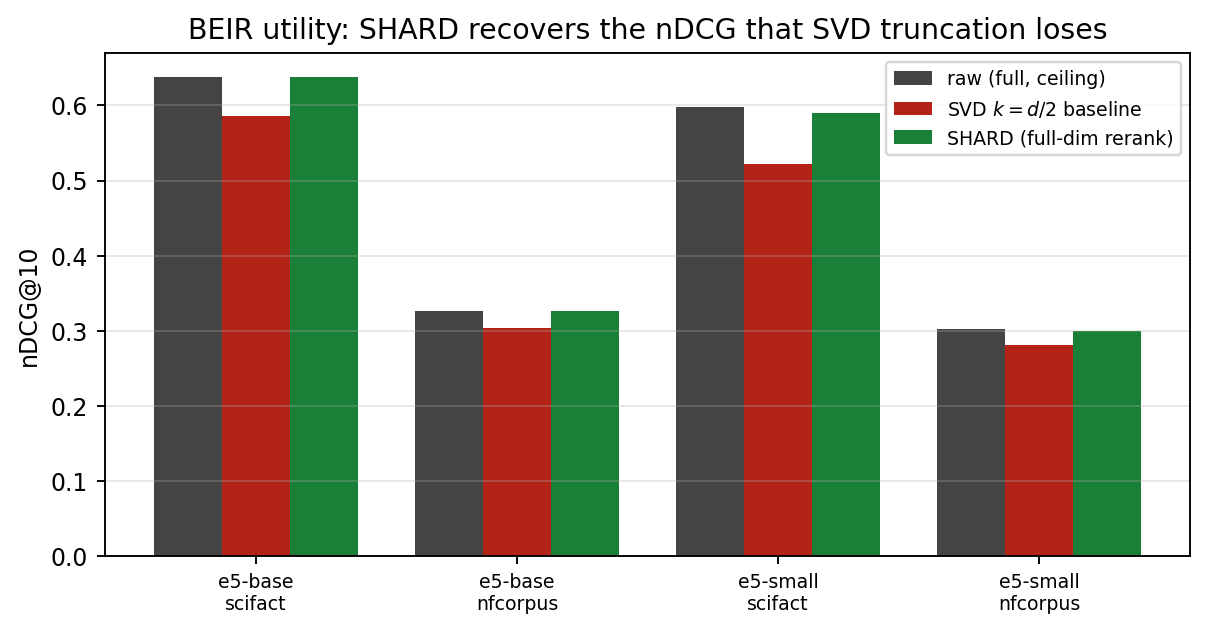
\includegraphics[width=0.74\linewidth]{fig_shard_beir.png}
\caption{BEIR utility: the SVD $k{=}d/2$ baseline loses nDCG@10 because it
reranks in the truncated half; \textsc{Shard} reranks full-dimensionally
and recovers the raw ceiling.}
\label{fig:shard-beir}
\end{figure}

% ----------------------------------------------------------------
\subsection{SHARD: online cost and the $C$ trade-off}\label{ssec:shard-cost}
% ----------------------------------------------------------------

\textsc{Shard} is not free relative to the single-query baseline, and we
measure the cost rather than assert it. The client sends one encrypted
residual query \emph{per active cell}---a cell touched by the stage-1
short-list---so the per-query upload and client-side encryption scale with
the number of distinct cells the short-list spans. Table~\ref{tab:shard-cost}
reports this directly. Two things matter. First, the absolute cost is
modest: even at $C{=}256$, $K_{\mathrm{cands}}{=}200$ the short-list spans
$\approx 30$ cells, i.e.\ $\approx 6$~MB of upload at one $0.21$~MB
ciphertext per cell, and the \emph{server} compute is unchanged
($\sim K_{\mathrm{cands}}$ ct-pt products, each scored with its cell's
keyed query) as is the download ($K_{\mathrm{cands}}$ score ciphertexts).
Second, and more important, this exposes the central trade-off of the
family: \emph{larger $C$ buys alignment resistance
(Section~\ref{ssec:shard-align}) but costs more active cells per query}. The
numbers are consistent across encoders (e5-base spans $\approx 9$--$35$
cells over the same grid). Active cells grow because $k$-means cells are
finer than a query's neighbourhood; a deployment tunes $(C,
K_{\mathrm{cands}}, d_{\mathrm{pub}})$ to balance alignment resistance,
stage-1 recall and upload, and the micro-key extreme ($C{=}N$) is the
endpoint where every candidate is its own cell ($\approx K_{\mathrm{cands}}$
queries).

\begin{table}[tbp]
\centering
\caption{\textsc{Shard} per-query online cost (e5-small, $d_{\mathrm{pub}}=d/4$).
Active cells set the upload (one $0.21$~MB ciphertext each); the baseline
($C{=}1$) sends one. Server compute and download are unchanged.}
\label{tab:shard-cost}
\small
\begin{tabular}{@{}lrrrr@{}}
\toprule
$K_{\mathrm{cands}}$ & \multicolumn{2}{c}{active cells (mean / p95)} & upload (MB) & $\times$ baseline\\
\cmidrule(lr){2-3}
 & $C{=}64$ & $C{=}256$ & ($C{=}256$) & ($C{=}256$)\\
\midrule
$40$  & $7.2 / 13$  & $11.6 / 19$ & $2.4$ & $11.6\times$\\
$100$ & $11.3 / 19$ & $20.0 / 32$ & $4.2$ & $20.0\times$\\
$200$ & $15.7 / 26$ & $30.1 / 48$ & $6.3$ & $30.1\times$\\
\bottomrule
\end{tabular}
\end{table}

% ----------------------------------------------------------------
\subsection{SHARD: alignment resistance scales with the cell count}\label{ssec:shard-align}
% ----------------------------------------------------------------

This is the central privacy result. We replicate the known-plaintext
alignment threat of Section~\ref{ssec:alignment-pq}, but against the
cell-keyed residual: an attacker holds $m$ pairs (native residual,
stored shard) and, for any cell with at least $d_{\mathrm{priv}}$ anchors,
solves orthogonal Procrustes to recover that cell's key, then de-keys and
re-identifies held-out targets in a $10\,000$-document residual gallery.
We use e5-small, $d_{\mathrm{pub}}=d/4=96$ ($d_{\mathrm{priv}}=288$), a
$200\,000$-document pool and $3$ seeds, and report the median/$90$th-percentile
anchor counts $m_{50},m_{90}$ for re-identification (Table~\ref{tab:shard-align},
Fig.~\ref{fig:shard-align}).

\begin{table}[tbp]
\centering
\caption{Alignment anchor-complexity (e5-small, $d_{\mathrm{priv}}=288$).
$m_{50}$ is the number of known-plaintext anchors at which residual
re-identification R@1 reaches $0.5$. Cell-local keys multiply the cost by
$\approx C$.}
\label{tab:shard-align}
\small
\begin{tabular}{@{}lrrr@{}}
\toprule
Scheme & residual keys & $m_{50}$ & factor vs.\ global \\ \midrule
global key (baseline) & $1$ over top-$k$ & $200$ & $1\times$ \\
\textsc{Shard} $C{=}1$ & $1$ over residual & $400$ & $2\times$ \\
\textsc{Shard} $C{=}64$ & $64$ cells & $25\,600$ & $128\times$ \\
\textsc{Shard} $C{=}256$ & $256$ cells & $102\,400$ & $512\times$ \\
\bottomrule
\end{tabular}
\end{table}

\begin{figure}[tbp]
\centering
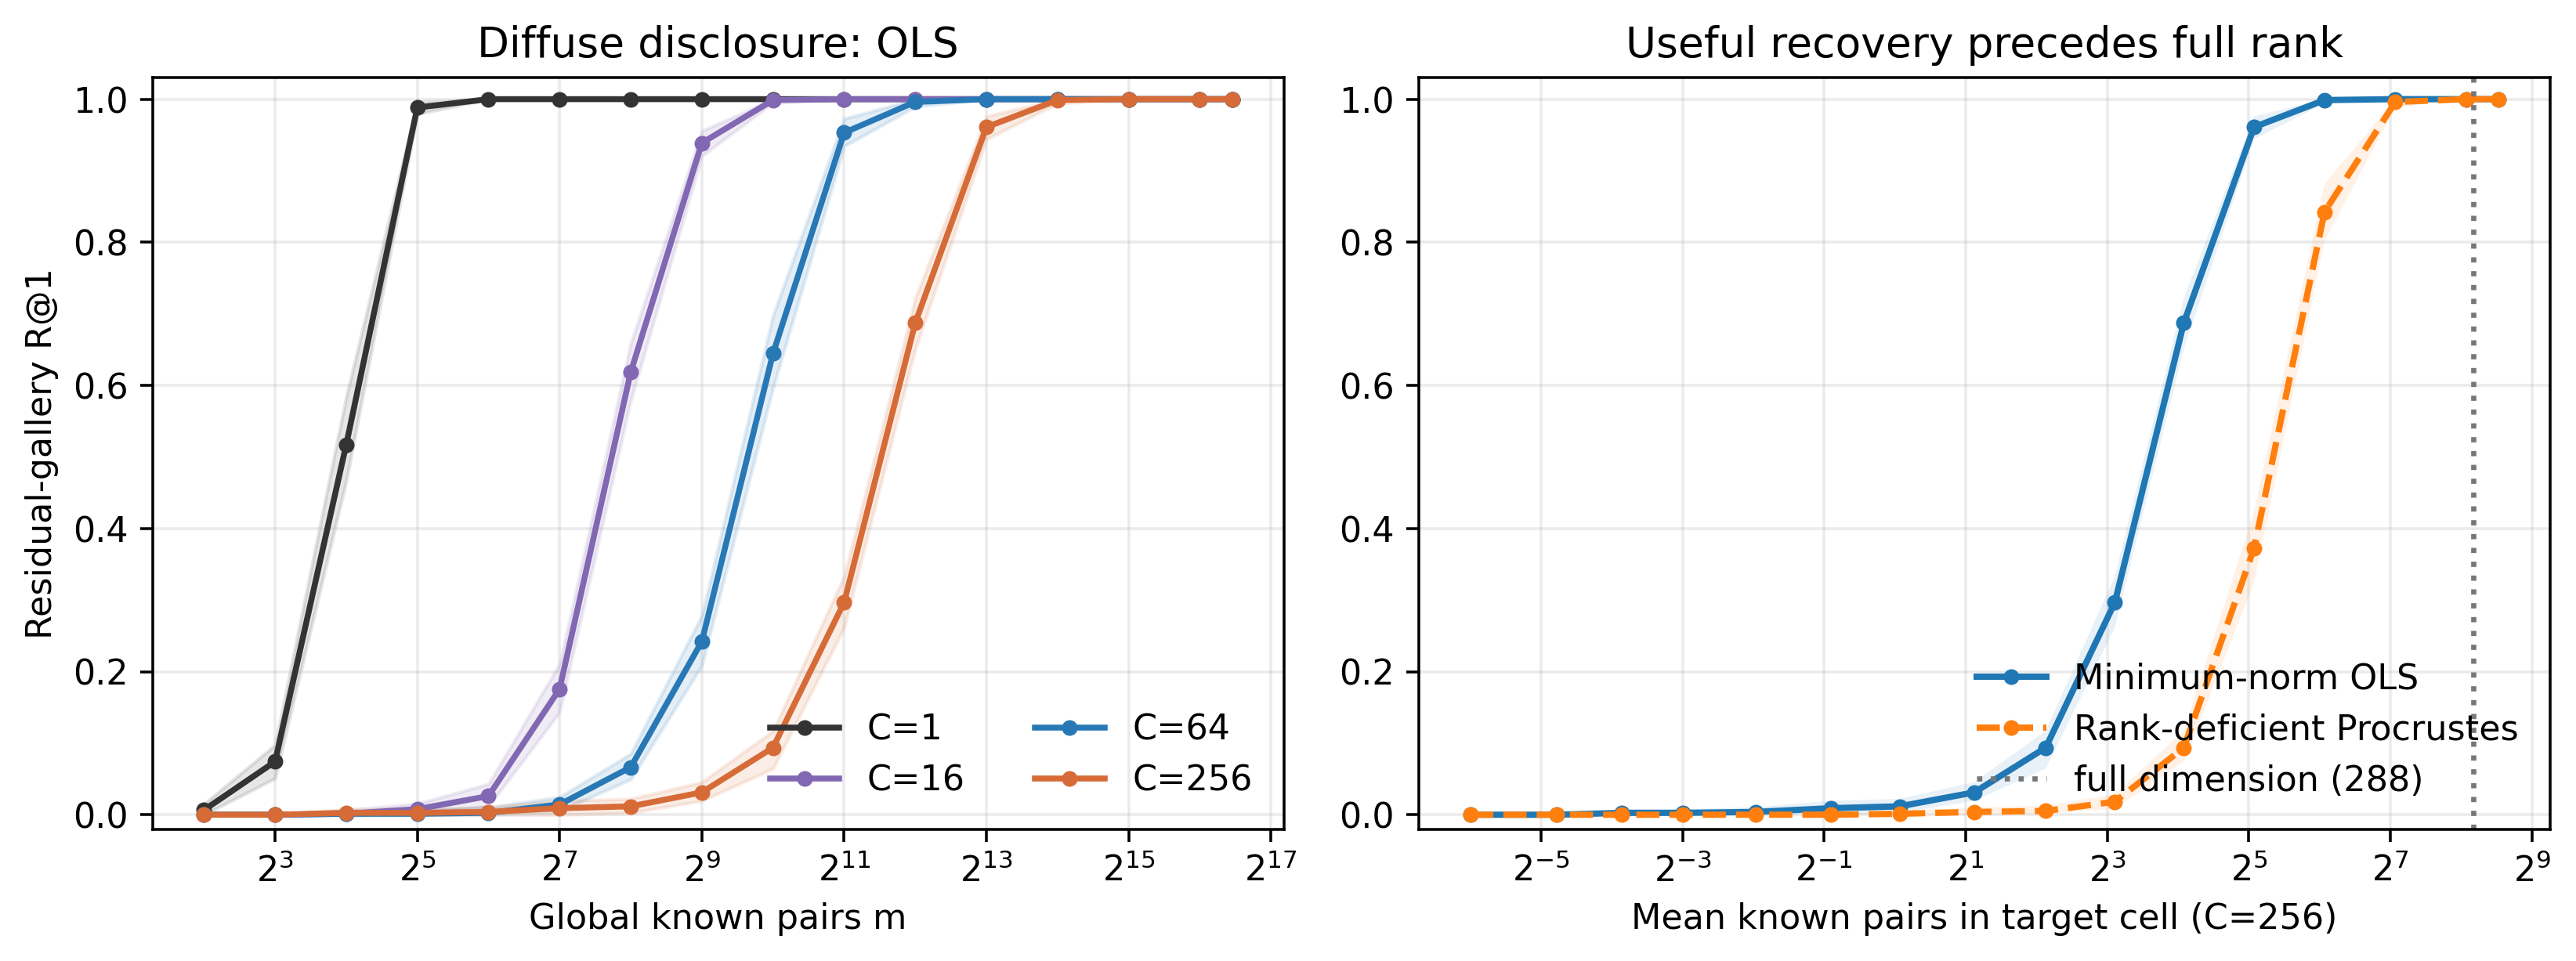
\includegraphics[width=0.72\linewidth]{fig_shard_alignment.png}
\caption{Residual re-identification R@1 vs.\ known-plaintext anchors $m$.
A single global key is recovered with $\sim d/2$ anchors; \textsc{Shard}
requires $\sim d_{\mathrm{priv}}$ anchors \emph{per cell}, shifting the
curve right by $\approx C$. The micro-key ($C{=}N$) limit is off-scale:
a per-document key cannot be recovered from other documents' anchors.}
\label{fig:shard-align}
\end{figure}

The scaling is clean and almost exactly linear in $C$: from $200$ anchors
for one global key, to $25\,600$ at $C{=}64$ and $102\,400$ at $C{=}256$
(a $512\times$ increase). The $C{=}1$ row already costs $2\times$ the
global baseline because \textsc{Shard} keys the \emph{whole} residual
($d_{\mathrm{priv}}{=}288$) rather than only the top-$k$ half, and the
transition is sharp---Procrustes either has enough in-cell anchors and
recovers the key exactly, or it does not---so $m_{50}\approx m_{90}$.
The result reproduces on a second encoder (e5-base, $d_{\mathrm{priv}}{=}576$):
$m_{50}$ grows from $400$ for the global key to $\sim\!51\,200$ at $C{=}64$,
again $\approx C\times$.

\paragraph{Diffuse vs.\ targeted leaks: what $\approx C$ does and does not
mean.} The $C\times$ factor is an \emph{aggregate} property: it is the cost
of recovering the store under a \emph{diffuse} known-plaintext leak whose
anchors fall uniformly across cells, so the median cell is saturated only
when the total reaches $\approx C\,d_{\mathrm{priv}}$. Because cells are
\emph{public}, a \emph{targeted} attacker can instead concentrate anchors
in a single victim's cell and recover only that key. We measure this
(Table~\ref{tab:shard-targeted}): targeted re-identification succeeds at
$\approx d_{\mathrm{priv}}$ in-cell anchors \emph{regardless of $C$}
($m_{50}^{\mathrm{tgt}}{=}320$ for e5-small at both $C{=}64$ and $C{=}256$,
versus $25\,600$/$102\,400$ diffuse). So the per-victim worst case is
$\approx d_{\mathrm{priv}}$---about $1.7\times$ the baseline's $d/2$, not
$C\times$---and \textsc{Shard}'s alignment advantage is precisely against
diffuse leaks and aggregate de-anonymisation of the store, plus the case
where a topically concentrated leak still cannot fill the victim's cell.
Two regimes make the targeted attack itself collapse: when an overlapping
plaintext reference exists, the public prefix already de-anonymises
(Section~\ref{ssec:shard-ref}), so the residual key is moot; and when cells
are smaller than $d_{\mathrm{priv}}$ (i.e.\ $C>N/d_{\mathrm{priv}}$, the
micro-key regime), no cell can supply $d_{\mathrm{priv}}$ in-cell anchors
and targeted recovery is impossible. The operational reading is that $C$
trades query cost (Section~\ref{ssec:shard-cost}) for diffuse-leak
resistance, while the micro-key limit is what removes the targeted
vulnerability outright.

\begin{table}[tbp]
\centering
\caption{Targeted attacker (anchors concentrated in the victim's public
cell). Re-identification needs $\approx d_{\mathrm{priv}}$ in-cell anchors
\emph{independently of $C$}---the $C\times$ factor is a diffuse-leak/aggregate
property, and the per-victim worst case is $\approx d_{\mathrm{priv}}$.}
\label{tab:shard-targeted}
\small
\begin{tabular}{@{}lrrr@{}}
\toprule
Encoder ($d_{\mathrm{priv}}$) & $m_{50}^{\mathrm{tgt}}$ ($C{=}64$) & $m_{50}^{\mathrm{tgt}}$ ($C{=}256$) & diffuse $m_{50}$ ($C{=}64$)\\
\midrule
e5-small ($288$) & $320$ & $320$ & $25\,600$\\
e5-base ($576$)  & $576$ & $576$ & $51\,200$\\
\bottomrule
\end{tabular}
\end{table}

% ----------------------------------------------------------------
\subsection{SHARD: stronger and learned alignment attackers}\label{ssec:shard-learned}
% ----------------------------------------------------------------

The $\approx C\times$ barrier was measured with orthogonal Procrustes; a
reviewer will rightly ask whether it is an artefact of assuming an
\emph{orthogonal} map. We therefore attack a single cell's keyed residual
($d_{\mathrm{priv}}{=}288$) with the alignment \emph{cores} of the modern
attacks and compare recovered-residual cosine vs in-cell anchors
(Fig.~\ref{fig:shard-learned}): a learned linear map (ridge least-squares,
the core of \textsc{ALGEN}'s few-shot alignment-and-generate
\cite{ref_algen}); a non-linear MLP; and unsupervised covariance/eigenvector
matching (the no-pairs core of \textsc{vec2vec}-style cross-space
translation \cite{ref_vec2vec}).

No attacker beats the $d_{\mathrm{priv}}$ barrier, and orthogonal Procrustes
is in fact the \emph{strongest} of the four. It exploits the known
orthogonality of $H_c$ and recovers the key \emph{exactly} at
$m=d_{\mathrm{priv}}$ (cosine $1.00$), with essentially nothing below it. The
learned linear map (\textsc{ALGEN} core) is \emph{weaker}: not constrained
to be orthogonal, it must fit $d_{\mathrm{priv}}^2$ free parameters and
reaches only cosine $0.68$ at $m=d_{\mathrm{priv}}$ and $0.80$ at $m=512$.
The MLP is worse still (cosine $\leq 0.13$): a non-linear hypothesis is the
wrong inductive bias for an orthogonal map and merely overfits. And the
unsupervised attacker fails outright (cosine $0.00$): the residual
covariance is anisotropic, so eigenvector matching pins down $H_c$ only up
to a per-axis \emph{sign}---a $2^{d_{\mathrm{priv}}}$ ambiguity that no
amount of unpaired data resolves. The anchor barrier is thus a property of
the construction---a $d_{\mathrm{priv}}$-dimensional secret orthogonal map
per cell---not of the particular attacker; the off-the-shelf Procrustes
used in Section~\ref{ssec:shard-align} is, if anything, the worst case for
the defender.

\begin{figure}[tbp]
\centering
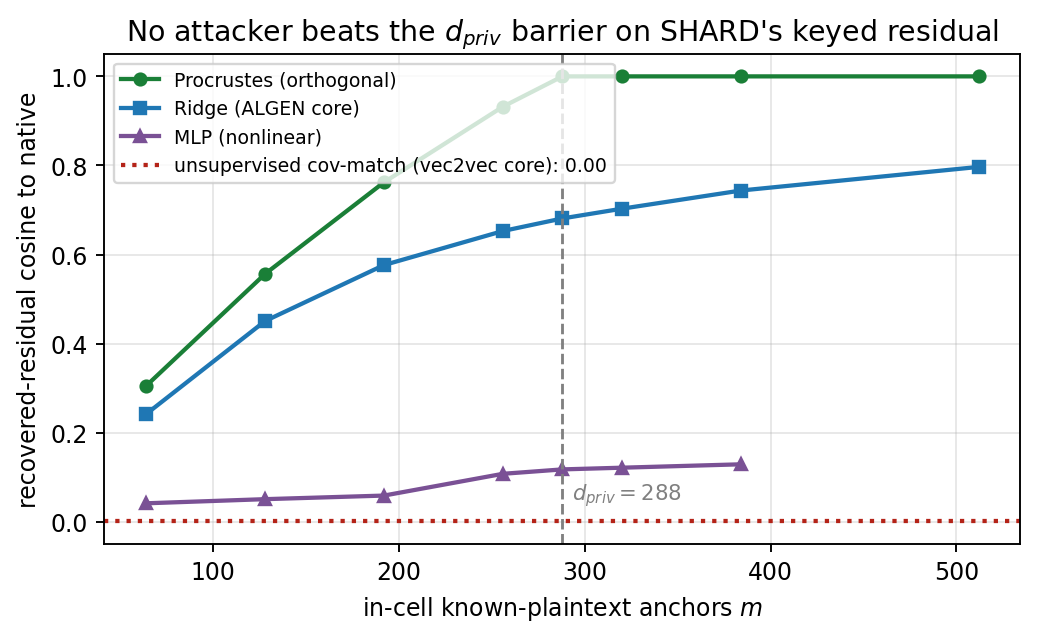
\includegraphics[width=0.68\linewidth]{fig_shard_learned.png}
\caption{Stronger attackers on \textsc{Shard}'s keyed residual. Recovered
cosine to the native residual vs in-cell anchors. Orthogonal Procrustes is
optimal (exact at $m=d_{\mathrm{priv}}$); the learned-linear \textsc{ALGEN}
core and an MLP are weaker; unsupervised \textsc{vec2vec}-style matching
fails (sign ambiguity). The barrier is not a Procrustes artefact.}
\label{fig:shard-learned}
\end{figure}

% ----------------------------------------------------------------
\subsection{SHARD: the public channel leaks coarse structure}\label{ssec:shard-leak}
% ----------------------------------------------------------------

The baseline's public PQ index sits on the full protected space and
preserves $67\%$ of exact top-10 neighbours (Section~\ref{ssec:alignment-pq}).
\textsc{Shard}'s public channel is only the short prefix $u$. We measure how
much true (full-space) top-10 neighbour structure each public channel
reveals (NN-overlap@10, e5-small, $100\,000$ documents, $1000$ probes;
Fig.~\ref{fig:shard-leak}). A $d/4$ prefix reveals NN-overlap $0.55$ and a
$d/8$ prefix only $0.36$ (and $0.20$ at $d/16$), against $0.76$ for the
baseline's exposed SVD $k{=}d/2$ geometry. The public stage-1 channel thus
discloses coarse/topic neighbours but not fine identity, which lives in the
keyed residual. The pattern reproduces on e5-base: a $d/8$ prefix leaks
NN-overlap $0.58$ and a $d/4$ prefix $0.77$, against $0.94$ for the
baseline geometry; the within-cell fraction is $0.55$/$0.46$ at
$C{=}64$/$256$.

\begin{figure}[tbp]
\centering
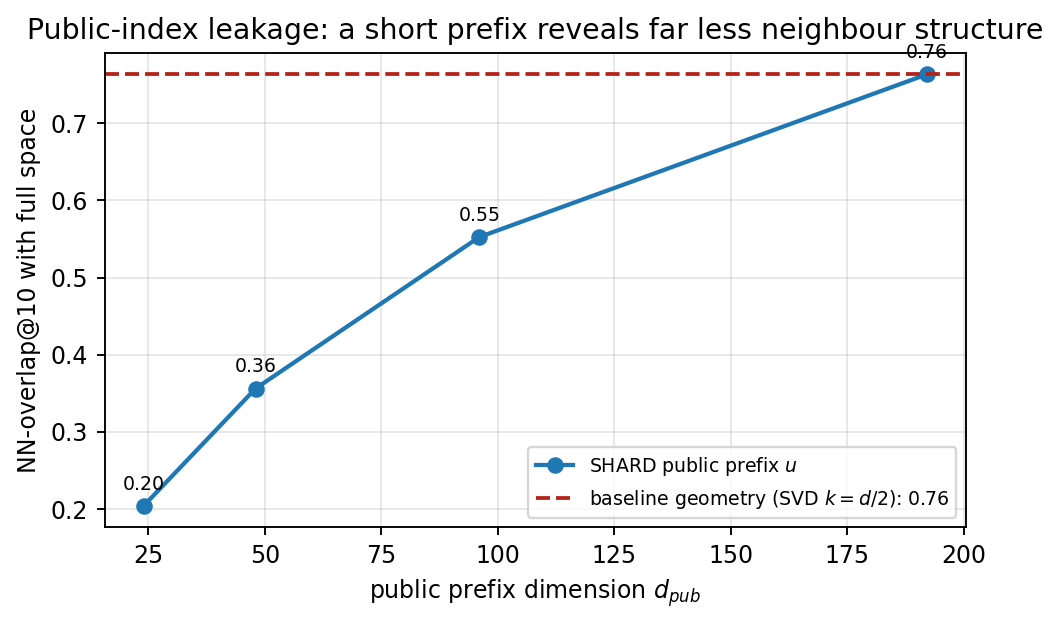
\includegraphics[width=0.66\linewidth]{fig_shard_leakage.png}
\caption{Public-index leakage (e5-small). The \textsc{Shard} public prefix
$u$ reveals far less of the true top-10 neighbour structure than the
baseline's exposed SVD $k{=}d/2$ geometry; a $d/8$ prefix discloses about
half as much.}
\label{fig:shard-leak}
\end{figure}

We are explicit about the residual leak. Within a cell the keys cancel, so
the server can compute exact same-cell similarities; the fraction of a
document's true top-10 neighbours that fall in its own cell---hence remain
recoverable---is $0.50$ at $C{=}64$ and $0.41$ at $C{=}256$, against $1.00$
for the baseline's single global key (which cancels for \emph{all} pairs).
More cells localise the leak further, and the micro-key variant removes it
entirely. \textsc{Shard} therefore shrinks, but does not zero, the
neighbour graph available to an honest-but-curious server.

% ----------------------------------------------------------------
\subsection{SHARD: the micro-key limit (no residual leak, unlinkable)}\label{ssec:shard-micro}
% ----------------------------------------------------------------

The within-cell residual leak and the targeted attack share one fix:
shrink cells to a single document. We measure the per-document micro-key
variant against the cell-level scheme (e5-small, $d_{\mathrm{pub}}=d/4$;
Table~\ref{tab:shard-micro}). The residual graph the server can reconstruct
from the keyed shards (the fraction of a document's true \emph{residual}
top-10 neighbours recoverable through same-key inner products) falls from
$0.25$ at $C{=}64$ to $0.18$ at $C{=}256$ and to $\mathbf{0.00}$ for
per-document keys---no two shards share a key, so no pairwise residual
similarity survives. And the residual channel is a genuine \emph{cancellable
template} \cite{ref_cancellable}: re-keying the store twice and trying to
match the same document across keys gives a mated-vs-non-mated AUC of
$\approx 0.50$ (cell $0.47$/$0.50$; micro-key $0.50$), i.e.\ renewable and
unlinkable. The price is bandwidth: micro-keys send one residual query per
candidate ($\approx K_{\mathrm{cands}}$ per search, the $C{=}N$ endpoint of
Table~\ref{tab:shard-cost}). The family therefore spans a clear spectrum:
cell-level \textsc{Shard} is the bandwidth-efficient operating point with
diffuse-leak resistance and a localised, non-zero residual leak;
per-document micro-keys are the high-assurance endpoint that removes the
residual leak \emph{and} the targeted attack, at $K_{\mathrm{cands}}$
queries per search. One honesty caveat carries over: unlinkability holds
for the \emph{residual} channel; the public prefix is identical across
re-keyings unless its global key is also refreshed
(Section~\ref{ssec:shard-ref}).

\begin{table}[tbp]
\centering
\caption{Micro-keys remove the residual leak and are unlinkable (e5-small).
Residual-graph recoverable: fraction of true residual top-10 neighbours the
server can reconstruct from the shards. Unlinkability AUC$\,{\approx}\,0.5$
means the same document is not matchable across two key sets.}
\label{tab:shard-micro}
\small
\begin{tabular}{@{}lrr@{}}
\toprule
Key granularity & residual-graph recoverable & unlinkability AUC \\ \midrule
cell, $C{=}64$ & $0.25$ & $0.47$ \\
cell, $C{=}256$ & $0.18$ & $0.50$ \\
micro-key (per-doc) & $\mathbf{0.00}$ & $0.50$ \\
\bottomrule
\end{tabular}
\end{table}

% ----------------------------------------------------------------
\subsection{SHARD vs.\ a distortion-aware defence}\label{ssec:shard-vs-dp}
% ----------------------------------------------------------------

\textsc{Shard} is \emph{attack-aware} (it keys the residual against
alignment) rather than \emph{distortion-aware} (adding noise calibrated to a
budget). To show the two are not interchangeable, we protect the \emph{same}
residual with calibrated isotropic Gaussian noise---a DP-style mechanism,
the natural lightweight alternative \cite{ref_lyu}---and place every defence
on the utility-vs-de-anonymisation plane (Table~\ref{tab:shard-vs-dp},
Fig.~\ref{fig:shard-vs-dp}). Utility is self-retrieval Acc@1; de-anonymisation
is a known-plaintext attacker's R@1 against a $10\,000$-document native
gallery at a diffuse budget of $m{=}400$ anchors.

The contrast is stark. \emph{DP-noise provides essentially no resistance to
this attack at any usable utility}: there is no transform to invert, so the
stored noised residual still matches its own native entry---de-anon R@1
stays $\geq0.996$ even at $\sigma{=}2\sigma_r$, where utility has already
fallen by six points, and only collapses once the noise is large enough to
destroy retrieval. A single global key (the $C{=}1$ baseline) is no better:
$m{=}400 > d_{\mathrm{priv}}$ anchors recover it, so de-anon R@1 $=1.0$.
\textsc{Shard} alone reaches the top-left corner: identical utility
($0.722$, the keyed rerank is exact) with de-anon R@1 $=0.00$, because a
diffuse budget of $400$ anchors cannot fill any cell. The mechanisms are
complementary---one could compose \textsc{Shard} with mild noise for
distortion on top of keying---but for the alignment/de-anonymisation surface
that the modern attacks target, keying is what pays.

\begin{table}[tbp]
\centering
\caption{Attack-aware vs.\ distortion-aware on the same residual (e5-small,
$d_{\mathrm{priv}}{=}288$). De-anon R@1 is a known-plaintext attacker against
a native gallery at $m{=}400$ diffuse anchors. Only \textsc{Shard} reaches
high utility \emph{and} low de-anonymisation.}
\label{tab:shard-vs-dp}
\small
\begin{tabular}{@{}lrr@{}}
\toprule
Defence (on the residual) & utility Acc@1 & de-anon R@1 ($m{=}400$)\\ \midrule
DP-noise $\sigma{=}0.25\sigma_r$ & $0.718$ & $1.00$ \\
DP-noise $\sigma{=}1.0\sigma_r$  & $0.711$ & $1.00$ \\
DP-noise $\sigma{=}2.0\sigma_r$  & $0.667$ & $1.00$ \\
global key ($C{=}1$)             & $0.722$ & $1.00$ \\
\textbf{\textsc{Shard} $C{=}64$} & $\mathbf{0.722}$ & $\mathbf{0.00}$ \\
\textbf{\textsc{Shard} $C{=}256$}& $\mathbf{0.722}$ & $\mathbf{0.00}$ \\
\bottomrule
\end{tabular}
\end{table}

\begin{figure}[tbp]
\centering
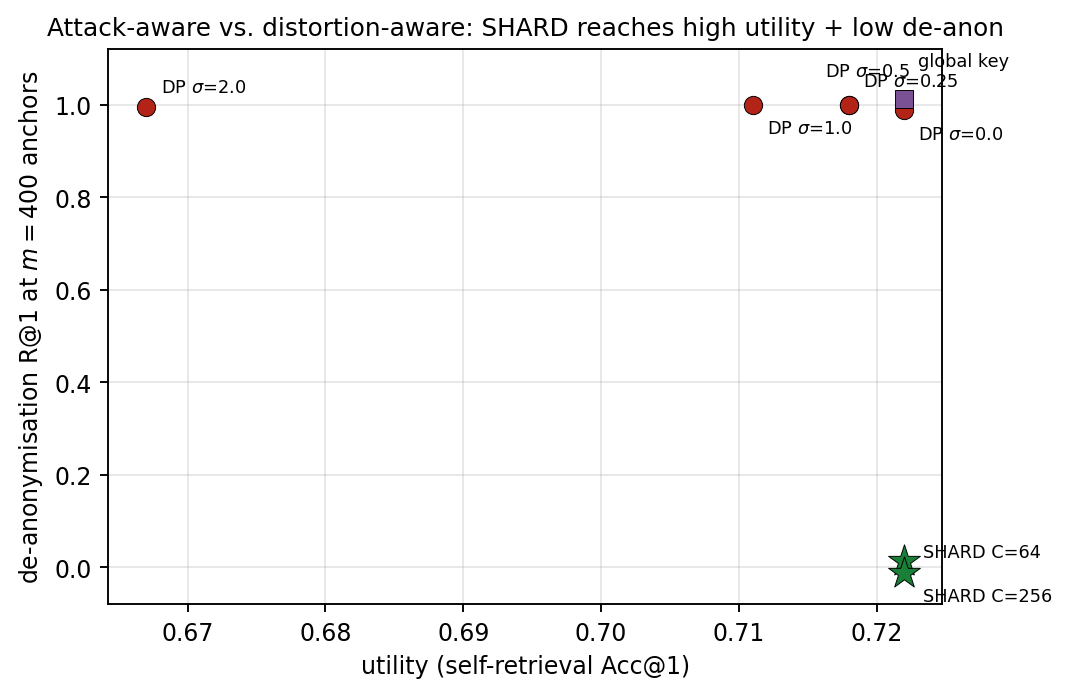
\includegraphics[width=0.66\linewidth]{fig_shard_vs_dp.png}
\caption{Utility vs.\ de-anonymisation at a fixed anchor budget. DP-noise
and a single global key sit at high de-anon (no alignment resistance);
\textsc{Shard} ($\star$) reaches high utility with near-zero
de-anonymisation.}
\label{fig:shard-vs-dp}
\end{figure}

% ----------------------------------------------------------------
\subsection{SHARD: a measured limitation (overlap reference lookup)}\label{ssec:shard-ref}
% ----------------------------------------------------------------

The baseline allowed an overlapping reference corpus to recover exact
source paragraphs after alignment ($99.8\%$ top-1,
Section~\ref{ssec:reference-attack}). We test whether \textsc{Shard} closes
this channel, keying both the prefix (one global key $K$) and the residual
(cell keys). It does \emph{not}, and we report this honestly. Because the
prefix carries a \emph{single} global key, it is recovered with only
$d_{\mathrm{pub}}$ anchors; once $K$ is known, the de-rotated public prefix
$u_t$ exactly matches the target's entry in an overlapping native reference,
so de-anonymisation R@1 stays near $1.0$ (e5-small, $100\,000$-document
reference: $0.995$ at $m{=}200$) regardless of the residual keys. In other
words, \textsc{Shard} hardens the \emph{native-frame mapping} of the private
residual (Section~\ref{ssec:shard-align}) but not the coarse identity
carried by an exposed prefix when the attacker already possesses the
plaintext. Two design responses follow directly: (i)~a \emph{coarse-cell-ID}
public channel, which exposes only the cell label (so overlap lookup
returns $\sim\!N/C$ candidates rather than one) at a stage-1 recall cost;
and (ii)~\emph{per-document micro-keys}, under which there is no global
prefix key to recover. We leave a full evaluation of these stronger
variants to future work and stress that \textsc{Shard}'s demonstrated
advantage is against alignment/inversion in the \emph{absence} of an
overlapping plaintext reference.

% =====================================================================
\FloatBarrier
\section{Discussion}\label{sec:discussion}
% =====================================================================

\paragraph{Why \textsc{Shard} is the right shape of defence.} The
measurements tell a consistent story. The baseline's protection is a
single global geometry, and every leakage channel we measured exploits
exactly that: Procrustes aligns the one rotation, the public PQ index sits
on the one space, and reference lookup follows once aligned. \textsc{Shard}
attacks the shape of the problem rather than adding noise to a surrogate:
it removes the global axis (cell keys), shrinks the public footprint to a
coarse prefix, and---by reranking the full residual rather than a truncated
half---actually \emph{improves} utility. The single knob $C$ turns the
\emph{diffuse}-leak known-plaintext cost from $O(d)$ into $O(Cd)$ and the
residual graph leak from global to cell-local, paying $\approx C$ extra
encrypted queries per search and leaving a per-victim targeted cost of
$\approx d_{\mathrm{priv}}$; the per-document limit removes the residual
leak and the targeted attack outright at $K_{\mathrm{cands}}$ queries. This
is the cancellable-template philosophy \cite{ref_cancellable} carried into
dense text retrieval: renewable, revocable, and tuned against attacks
rather than against $\sigma_{rec}$---with the trade-offs measured rather
than assumed. The contrast with the distortion-aware alternative is the
cleanest evidence for this stance: at matched utility a DP-noise residual
is still trivially de-anonymised (R@1 $\approx 1$), because noise has no key
to recover, whereas \textsc{Shard}'s keyed residual is not---and the keying
holds against learned-linear, non-linear and unsupervised attackers, not
just the orthogonal Procrustes that motivated it.

\paragraph{Encoder selection is part of the protocol.} The baseline
protective wrapper is essentially metric-preserving in the projected
space; the
end-to-end deviation from the raw baseline is dominated by what
end-to-end deviation from the raw baseline is dominated by what
SVD truncation does on the chosen encoder. Models trained with
contrastive retrieval objectives and large dimension
(\textsc{e5-large}, \textsc{bge-m3}, $d{=}1024$) concentrate the retrieval
signal in the top singular directions: half truncation leaves Acc@1
unchanged (no significant difference) and \emph{significantly} improves
Acc@10 (Section~\ref{ssec:significance}), the linear-denoiser effect.
The mid-sized \textsc{e5-base} ($d{=}768$) is statistically
indistinguishable from raw. Paraphrase-distilled models (\textsc{mpnet})
and very compact models (\textsc{e5-small}, $d{=}384$) do \emph{not} show
this concentration: truncation significantly degrades retrieval, so we
recommend either replacing them with a retrieval-trained $d\geq 1024$
equivalent or running a $k$-sweep before deployment to find a $k$ that
satisfies both the application's accuracy budget and the
$\sigma_{rec}\geq 0.10$ distortion floor.

\paragraph{The role of the rotation $R$: obfuscation, not a primitive.}
We state this as plainly as possible: \emph{the secret rotation is an
empirical obfuscation layer, not a cryptographic primitive}. It
contributes a defence channel orthogonal to SVD truncation, and even at
$k/d = 1.0$ the unknown-$R$ regime reduces off-the-shelf Vec2Text BLEU
to the noise floor---but the paper also reports that a known-$R$ attacker
gains nothing beyond SVD and that a known-plaintext attacker recovers the
orientation with standard Procrustes alignment. The aligned Vec2Text
stress test does not recover text or typed PII, but its raw baseline is
already near the reconstruction floor; a learned or universal decoder
adapted to the protected space is still untested and out of scope. The
rotation's value proposition is therefore limited: it is a cheap obstacle
for a weak unknown-orientation attacker, not a security guarantee. The
scientific weight of the paper is the measured privacy/latency/accuracy
trade-off and the documented failure modes, not the rotation.

\paragraph{What CKKS hides and what it does not.} The CKKS layer hides
the numerical representation of the query and the exact similarity
scores from the server. Two things it does \emph{not} hide are the
identifiers of the candidates produced by stage-1 PQ filtering and the
$L_2$-distances among them implicit in the order in which they are
sent. Section~\ref{ssec:alignment-pq} also shows that the public PQ
codes preserve substantial local geometry even before observing queries.
An access-pattern attacker can therefore, over many queries, build a
co-occurrence model of which documents are co-retrieved.
Composing the pipeline with a PIR-style retrieval primitive (Tiptoe
\cite{ref_tiptoe}, SealPIR \cite{ref_sealpir}, OnionPIR
\cite{ref_onionpir}, SimplePIR \cite{ref_simplepir}) is the natural
remedy; ours is engineered to be PIR-friendly because the
ct-pt operations on the server are stateless and cluster-local.

\paragraph{Parameter selection.} The selected configuration is
$\approx 1.7\times$ faster than the TenSEAL stock parameters at the same
parameter-table security bound and within $\Delta\mathrm{Acc@1}\leq 1$~p.p.\
of baseline\_proj. We reiterate that this speed-up is structural---ct-pt
needs one multiplicative level, hence a shorter modulus chain---rather than
a product of the learned surrogate, which only serves to extrapolate
latency to unbenchmarked configurations or hardware. The selection runs
offline at no per-query cost.

% =====================================================================
\section{Limitations and Future Work}\label{sec:limits}
% =====================================================================

We separate \emph{intrinsic limitations} (properties of the construction
under study) from \emph{future work} (experiments that would extend the
measurement, especially before any \emph{security} claim could be made for
a security venue). We name and scope the latter rather than leaving it
vague, so the boundary of what we measured is explicit.

\paragraph{Intrinsic limitations.}
\begin{itemize}[leftmargin=18pt,topsep=2pt,itemsep=2pt]
\item \emph{\textsc{Shard} hardens alignment, not the coarse graph.} The
keyed residual resists native-frame mapping ($\approx C\times$ anchors),
but two channels remain: within a cell the keys cancel, so same-cell
similarities leak ($0.50$ of the neighbour graph at $C{=}64$); and the
public prefix, carrying a single global key, is recovered with
$d_{\mathrm{pub}}$ anchors, after which an \emph{overlapping} reference
corpus de-anonymises through it (Section~\ref{ssec:shard-ref}). The
micro-key and coarse-cell-ID variants address these at a bandwidth or
recall cost but are not yet evaluated.
\item \emph{\textsc{Shard} is a geometric, not cryptographic, defence.} It
is an attack-aware transform with measured advantages against alignment and
index leakage; it carries no formal privacy guarantee, and like the
baseline it leaves access patterns to a PIR/ORAM composition.
\item \emph{Baseline: document privacy is not cryptographic.} $E_{\mathrm{rot}}$
is plaintext on the server; it is protected only by SVD truncation (a
proxy) and the secret rotation (an empirical obfuscation layer).
Section~\ref{ssec:alignment-pq} shows that known plaintext anchors
defeat the rotation by standard alignment, and
Section~\ref{ssec:reference-attack} shows that an overlapping reference
corpus can then recover the exact source paragraph.
\item \emph{Access patterns and PQ codes are exposed.} CKKS hides values,
not which candidates are reranked, and the public PQ codes are a lossy
view of $E_{\mathrm{rot}}$. The measured PQ-code leakage is
non-negligible; production use requires composition with a PIR/ORAM layer
and a static-side protection for the public index artefact.
\item \emph{Encoder-dependence of the accuracy budget.} The strict
end-to-end criterion $\Delta\mathrm{Acc@1} \geq -5$~p.p.\ holds only
on retrieval-trained encoders with $d \geq 768$. Compact or
paraphrase-distilled encoders need either replacement or a less
aggressive $k$ (which then violates the $\sigma_{rec} \geq 0.10$ proxy).
\item \emph{Scale vs.\ task realism.} The $10^6$-scale experiment is a
self-retrieval geometry probe on Russian Wikipedia---a strong
transform-fidelity test, not a production IR benchmark. The BEIR experiment
(Section~\ref{ssec:beir}) shows that the denoiser effect seen on that probe
does \emph{not} transfer to real graded-relevance tasks; but BEIR itself
is evaluated only at the few-thousand-document scale of SciFact/NFCorpus
and only for the e5 family. The cleanest remaining test---a real,
$10^6$-scale, multilingual IR benchmark with graded qrels---was beyond our
CPU encoding budget and remains future work; it would resolve whether the
self-retrieval/real-IR gap is driven by corpus \emph{scale} or by task
\emph{structure}.
\item \emph{Generative inversion calibration is corpus- and model-limited.}
The aligned Vec2Text stress test uses an offline synthetic-news+PII corpus
and an off-the-shelf corrector; because raw inversion is already weak, the
zero PII-recall result should be read as a boundary condition for this
attacker, not as general document privacy.
\item \emph{Single-machine evaluation.} The latency numbers in
Section~\ref{ssec:latency} are taken on loopback HTTP; a
geographically distributed deployment will add (uncharacterised)
network latency.
\end{itemize}

\paragraph{Future work.}
\begin{enumerate}[leftmargin=20pt,topsep=2pt,itemsep=3pt]
\item \emph{The stronger \textsc{Shard} variants (highest priority).}
Evaluate the per-document micro-key and coarse-cell-ID channels that close
the within-cell and overlap-reference-lookup leaks identified in
Sections~\ref{ssec:shard-leak}--\ref{ssec:shard-ref}, quantifying their
bandwidth (extra residual queries) and stage-1 recall costs, and a learned
per-cell key schedule.
\item \emph{Full generative pipelines against \textsc{Shard}.}
Section~\ref{ssec:shard-learned} stress-tests the \emph{alignment cores} of
\textsc{ALGEN} (learned linear), \textsc{vec2vec} (unsupervised) and a
non-linear MLP, and the barrier holds. The remaining work needs a GPU: the
full generative stages---\textsc{ALGEN}'s text generator and
\textsc{ZSInvert}'s zero-shot LLM decoder---and a decoder fine-tuned on
protected embeddings, to confirm that failing to recover the native
residual also fails to recover text.
\item \emph{Learned adaptive-decoder attack on the baseline.}
Section~\ref{ssec:adaptive-inversion} evaluates aligned off-the-shelf
Vec2Text, not a decoder fine-tuned on rotated/SVD embeddings. The
decisive remaining text-level test is to train or fine-tune an inversion
model on protected embeddings from part of the corpus and evaluate
BLEU, token overlap and typed-PII recovery on a disjoint holdout.
\item \emph{Per-encoder $\sigma_{rec}$ vs.\ text leakage ablation.}
Section~\ref{ssec:projection-baselines} now includes a geometry-level
diagnostic showing that $\sigma_{rec}$ is not itself a privacy metric.
The remaining required experiment is text-level: replace the
single-encoder, BLEU-only calibration of the $\sigma_{rec}=0.10$ proxy
with a multi-encoder ablation reporting BLEU, token overlap and typed-PII
recovery (names, addresses, e-mail, phone, medical terms).
\item \emph{Stronger baseline suite.} Extend the lightweight baseline
analysis beyond the calibrated Gaussian-noise diagnostic to
quantisation/noise mechanisms with formal DP budgets and accuracy-matched
operating points. The present paper includes SVD, Gaussian random
projection, random orthogonal projection and matched-distortion
independent Gaussian noise.
\item \emph{Benchmark generality at scale.} Section~\ref{ssec:beir} shows
that the denoiser \emph{fails} to transfer to BEIR SciFact/NFCorpus
(SVD significantly reduces nDCG@10). The remaining work is to test whether
the self-retrieval/real-IR gap is driven by corpus \emph{scale} or task
\emph{structure}, using larger multilingual IR benchmarks (MIRACL,
MS~MARCO) at $10^6$ scale---where CPU encoding was the binding constraint
here---and a GPU-encoded e5-large/NFCorpus cell to complete the grid.
\item \emph{Stronger universal inverter configuration.} Repeat
Sections~\ref{ssec:vec2text} and~\ref{ssec:adaptive-inversion} with beam
search, many more corrector iterations and a modern universal/zero-shot
inversion model, so the ``BLEU at noise floor'' statement is not tied to
the evaluated off-the-shelf corrector.
\item \emph{Disjoint-reference and cross-space transfer attacks.}
Section~\ref{ssec:reference-attack} evaluates the overlap case. The
remaining stress tests are harder: non-overlapping external corpora,
semantic judges for near-neighbour leakage, and embedding-space
translation attacks such as vec2vec-style mappings. The known-plaintext
experiment shows that linear alignment can be damaging; unsupervised or
weakly supervised alignment remains untested.
\end{enumerate}

% =====================================================================
\section{Conclusion}\label{sec:conclusion}
% =====================================================================

We began by measuring a popular global-linear defence for private dense
retrieval---SVD truncation, a secret rotation, a public ANN index and CKKS
reranking---and found its protection concentrated on a single weak axis. A
known-plaintext orthogonal Procrustes attack recovers the secret rotation
with about $k=d/2$ anchors; an overlapping reference corpus then yields
near-exact paragraph recovery; the public product-quantisation index
preserves most of the neighbour structure; and, because reranking happens
in the truncated half, the stack loses $2$--$8$ nDCG@10 points on BEIR. The
distortion proxy $\sigma_{rec}$ that such schemes optimise is, as our
calibrated-noise diagnostic confirms, not a privacy metric at all. These
are precisely the openings that modern alignment, zero-shot inversion and
cross-space translation attacks exploit.

\textsc{Shard} removes the weak axis. By splitting the embedding into a
coarse public prefix and a private residual that is sharded into $C$
cell-keyed pieces, it (i)~recovers raw retrieval quality---reranking is
full-dimensional, so it matches the raw nDCG@10 that truncation drops on
BEIR while exposing a public channel half as wide; (ii)~multiplies the
diffuse known-plaintext anchor complexity of mapping the store back to the
native frame by $\approx C$ (from $200$ to $102{,}400$ anchors at
$C{=}256$, holding against learned-linear, non-linear and unsupervised
attackers, where a matched-utility DP-noise defence offers no resistance at
all); and (iii)~confines the public index to coarse, topic-level neighbours
and localises the residual neighbour-graph leak to cells, both shrinking
with $C$ and vanishing at the per-document micro-key limit. A single parameter $C$ tunes the family from the global baseline
($C{=}1$) to per-document micro-keys ($C{=}N$), and re-keying a cell gives
revocation at cell granularity.

We are equally clear about what \textsc{Shard} does \emph{not} do. It
hardens the alignment and index-leakage surface, not the coarse graph:
within a cell the keys cancel, and an overlapping plaintext reference still
de-anonymises through the single-keyed public prefix. It is an attack-aware
\emph{geometric} transform, not a cryptographic guarantee, and it inherits
the baseline's open access-pattern channel. Closing the residual graph and
the overlap channel with the micro-key and coarse-cell-ID variants,
stress-testing \textsc{Shard} against learned and zero-shot inverters, and
composing it with a PIR-style access-pattern hider are the natural next
steps. The contribution here is to move embedding privacy from a single
alignable geometry, optimised against a distortion surrogate, to a
\emph{family} of cell-keyed transforms whose advantage against the modern
attack surface is measured rather than assumed.

% =====================================================================
\section*{Reproducibility}
% =====================================================================

All code, configuration, and the JSON/CSV outputs of every experiment are
released as a structured repository. It is organised into \path{shard/}
(the contribution: \path{shard_lib.py} and the eleven \texttt{exp12}--%
\texttt{exp22} scripts for utility, online cost, alignment resistance
(diffuse, targeted and against learned/unsupervised attackers),
public-index leakage, the micro-key variant, the DP-noise comparison and
the reference-lookup limitation), \path{baseline/} (the global-linear foil:
the integral $10^6$-document pipeline, the Procrustes/PQ leakage, the
$\sigma_{rec}$ diagnostic, the denoiser-significance and BEIR experiments,
and the GPU Vec2Text stress test), \path{results/} (one directory per
experiment), \path{paper/}, and \path{docs/}. The \textsc{Shard} and
lightweight-baseline experiments are \texttt{numpy}/\texttt{scikit-learn}
only---the per-cell keys are orthogonal, so the residual reranking score is
exact and is computed directly, needing no FHE library---except the BEIR
encoding (CPU \texttt{torch}) and the optional GPU stress test. All runs are
deterministic given their seeds (query/ground-truth seed $42$, rotation and
master-key seeds $\{11,23,31,47,53\}$, bootstrap seed $2026$). The cached
embeddings (one-million Russian-Wikipedia paragraphs for five encoders,
reproducibly sliced from a public dump with the date and checksum in the
data manifest; $\approx\!17$~GB) are not shipped with the repository and are
located through a \texttt{SHARD\_DATA} path; the BEIR data is the public
\texttt{BeIR/scifact} and \texttt{BeIR/nfcorpus} releases. A public DOI
archive and target-journal data statement remain to be added before formal
submission.

% =====================================================================
\begin{thebibliography}{99}\small
% =====================================================================

\bibitem{ref_sbert} N.\ Reimers and I.\ Gurevych, ``Sentence-BERT:
Sentence Embeddings using Siamese BERT-Networks,'' in
\emph{Proc.\ EMNLP}, 2019, pp.\ 3982--3992.

\bibitem{ref_e5} L.\ Wang, N.\ Yang, X.\ Huang, et al.,
``Text Embeddings by Weakly-Supervised Contrastive Pre-training,''
\emph{arXiv:2212.03533}, 2022.

\bibitem{ref_gtr} J.\ Ni et al., ``Large Dual Encoders Are Generalizable
Retrievers,'' in \emph{Proc.\ EMNLP}, 2022, pp.\ 9844--9855.

\bibitem{ref_bgem3} J.\ Chen, S.\ Xiao, P.\ Zhang, K.\ Luo, D.\ Lian,
and Z.\ Liu, ``BGE M3-Embedding: Multi-Lingual, Multi-Functionality,
Multi-Granularity Text Embeddings Through Self-Knowledge Distillation,''
\emph{arXiv:2402.03216}, 2024.

\bibitem{ref_dpr} V.\ Karpukhin et al., ``Dense Passage Retrieval for
Open-Domain Question Answering,'' in \emph{Proc.\ EMNLP}, 2020,
pp.\ 6769--6781.

\bibitem{ref_colbert} O.\ Khattab and M.\ Zaharia, ``ColBERT: Efficient
and Effective Passage Search via Contextualised Late Interaction over
BERT,'' in \emph{Proc.\ ACM SIGIR}, 2020, pp.\ 39--48.

\bibitem{ref_vec2text} J.\ X.\ Morris, V.\ Kuleshov, V.\ Shmatikov, and
A.\ M.\ Rush, ``Text Embeddings Reveal (Almost) As Much As Text,'' in
\emph{Proc.\ EMNLP}, 2023.

\bibitem{ref_geia} J.\ Gu et al., ``GEIA: Gradient-based Embedding
Inversion Attack,'' \emph{arXiv:2304.08945}, 2023.

\bibitem{ref_teia} X.\ Pan et al., ``TEIA: Text Embedding Inversion
Attacks,'' \emph{arXiv:2305.08450}, 2023.

\bibitem{ref_algen} Y.\ Chen, Q.\ Xu, and J.\ Bjerva, ``ALGEN:
Few-shot Inversion Attacks on Textual Embeddings via Cross-Model
Alignment and Generation,'' in \emph{Proc.\ ACL}, 2025.

\bibitem{ref_zsinvert} Y.\ Zhang, J.\ X.\ Morris, and V.\ Shmatikov,
``Universal Zero-shot Embedding Inversion,'' \emph{arXiv:2504.00147},
2025.

\bibitem{ref_lago} Y.\ Yu et al., ``LAGO: Few-shot Crosslingual
Embedding Inversion Attacks via Language Similarity-Aware Graph
Optimization,'' \emph{arXiv:2505.16008}, 2025.

\bibitem{ref_eguard} T.\ Liu et al., ``EGuard: Defending LLM Embeddings
Against Inversion Attacks via Text Mutual Information Optimization,''
in \emph{Proc.\ AAAI}, 2026.

\bibitem{ref_sparse} Y.-C.\ Tsai, H.\ Hsiao, K.-Y.\ Chen, and S.-D.\
Lin, ``Concept-Aware Privacy Mechanisms for Defending Embedding
Inversion Attacks,'' in \emph{Proc.\ ICLR}, 2026.

\bibitem{ref_nvdp} D.\ El Zein, S.\ Kumar, and J.\ Henderson,
``Nonparametric Variational Differential Privacy via Embedding Parameter
Clipping,'' \emph{arXiv:2603.09583}, 2026.

\bibitem{ref_mrl} A.\ Kusupati et al., ``Matryoshka Representation
Learning,'' in \emph{Advances in Neural Information Processing Systems},
2022.

\bibitem{ref_vec2vec} R.\ Jha, C.\ Zhang, V.\ Shmatikov, and J.\ X.\
Morris, ``Harnessing the Universal Geometry of Embeddings,''
\emph{arXiv:2505.12540}, 2025.

\bibitem{ref_zeng_rag} S.\ Zeng et al., ``The Good and the Bad:
Exploring Privacy Issues in Retrieval-Augmented Generation (RAG),''
in \emph{Findings of ACL}, 2024, pp.\ 4505--4524.

\bibitem{ref_song_leak} C.\ Song and A.\ Raghunathan, ``Information
Leakage in Embedding Models,'' in \emph{Proc.\ ACM CCS}, 2020,
pp.\ 377--390.

\bibitem{ref_shokri} R.\ Shokri et al., ``Membership Inference Attacks
Against Machine Learning Models,'' in \emph{Proc.\ IEEE S\&P},
2017, pp.\ 3--18.

\bibitem{ref_carlini} N.\ Carlini et al., ``Extracting Training Data
from Large Language Models,'' in \emph{Proc.\ USENIX Security},
2021, pp.\ 2633--2650.

\bibitem{ref_dwork} C.\ Dwork, ``Differential Privacy,'' in
\emph{Proc.\ ICALP}, 2006, pp.\ 1--12.

\bibitem{ref_dpsgd} M.\ Abadi et al., ``Deep Learning with Differential
Privacy,'' in \emph{Proc.\ ACM CCS}, 2016, pp.\ 308--318.

\bibitem{ref_lyu} L.\ Lyu, X.\ He, and Y.\ Li, ``Differentially Private
Representation for NLP,'' in \emph{Findings of EMNLP}, 2020,
pp.\ 2355--2365.

\bibitem{ref_kenthapadi} K.\ Kenthapadi, A.\ Korolova, I.\ Mironov, and
N.\ Mishra, ``Privacy via the Johnson-Lindenstrauss Transform,''
\emph{J.\ Privacy and Confidentiality}, vol.\ 5, no.\ 1, 2013.

\bibitem{ref_liu} K.\ Liu, H.\ Kargupta, and J.\ Ryan,
``Random Projection-Based Multiplicative Data Perturbation for Privacy
Preserving Distributed Data Mining,'' \emph{IEEE TKDE}, vol.\ 18,
no.\ 1, 2006, pp.\ 92--106.

\bibitem{ref_ckks} J.\ H.\ Cheon, A.\ Kim, M.\ Kim, and Y.\ Song,
``Homomorphic Encryption for Arithmetic of Approximate Numbers,'' in
\emph{Advances in Cryptology---ASIACRYPT 2017}, LNCS 10624, pp.\ 409--437.

\bibitem{ref_ckks_bootstrap} J.\ H.\ Cheon, K.\ Han, A.\ Kim et al.,
``Bootstrapping for Approximate Homomorphic Encryption,'' in
\emph{Advances in Cryptology---EUROCRYPT 2018}, LNCS 10820,
pp.\ 360--384.

\bibitem{ref_he_std} M.\ Albrecht et al., ``Homomorphic Encryption
Security Standard,'' HomomorphicEncryption.org, 2018.

\bibitem{ref_lwe_estimator} M.\ R.\ Albrecht, R.\ Player, and S.\ Scott,
``On the Concrete Hardness of Learning with Errors,'' \emph{Journal of
Mathematical Cryptology}, vol.\ 9, no.\ 3, 2015, pp.\ 169--203
(lattice-estimator methodology).

\bibitem{ref_schonemann} P.\ H.\ Sch\"onemann, ``A Generalized Solution
of the Orthogonal Procrustes Problem,'' \emph{Psychometrika}, vol.\ 31,
no.\ 1, 1966, pp.\ 1--10.

\bibitem{ref_cancellable} V.\ M.\ Patel, N.\ K.\ Ratha, and R.\ Chellappa,
``Cancelable Biometrics: A Review,'' \emph{IEEE Signal Processing
Magazine}, vol.\ 32, no.\ 5, 2015, pp.\ 54--65.

\bibitem{ref_openfhe} A.\ Al Badawi et al., ``OpenFHE: Open-Source Fully
Homomorphic Encryption Library,'' in \emph{Proc.\ WAHC '22},
2022, pp.\ 53--63.

\bibitem{ref_eva} R.\ Dathathri et al., ``EVA: An Encrypted Vector
Arithmetic Language and Compiler for Efficient Homomorphic
Computation,'' in \emph{Proc.\ ACM PLDI}, 2020, pp.\ 546--561.

\bibitem{ref_chet} R.\ Dathathri et al., ``CHET: An Optimizing Compiler
for Fully-Homomorphic Neural-Network Inferencing,'' in
\emph{Proc.\ ACM PLDI}, 2019, pp.\ 142--156.

\bibitem{ref_jung_gpu} W.\ Jung, S.\ Kim, J.\ H.\ Ahn et al.,
``Over 100x Faster Bootstrapping in Fully Homomorphic Encryption
through Memory-centric Optimisation with GPUs,'' \emph{IACR TCHES},
vol.\ 2021, no.\ 4, pp.\ 114--148.

\bibitem{ref_hexl} F.\ Boemer et al., ``Intel HEXL: Accelerating
Homomorphic Encryption with Intel AVX512-IFMA52,'' in
\emph{Proc.\ WAHC '21}, 2021, pp.\ 57--62.

\bibitem{ref_tiptoe} A.\ Henzinger, E.\ Dauterman, H.\ Corrigan-Gibbs,
and N.\ Zeldovich, ``Private Web Search with Tiptoe,'' in
\emph{Proc.\ ACM SOSP}, 2023.

\bibitem{ref_sealpir} S.\ Angel, H.\ Chen, K.\ Laine, and S.\ Setty,
``PIR with Compressed Queries and Amortised Query Processing,'' in
\emph{Proc.\ IEEE S\&P}, 2018, pp.\ 962--979.

\bibitem{ref_simplepir} A.\ Henzinger, M.\ M.\ Hong, H.\ Corrigan-Gibbs,
S.\ Meiklejohn, and V.\ Vaikuntanathan, ``One Server for the Price of
Two: Simple and Fast Single-Server Private Information Retrieval
(SimplePIR),'' in \emph{Proc.\ USENIX Security}, 2023.

\bibitem{ref_onionpir} M.\ H.\ Mughees, H.\ Chen, and L.\ Ren,
``OnionPIR: Response Efficient Single-Server PIR,'' in
\emph{Proc.\ ACM CCS}, 2021, pp.\ 2292--2306.

\bibitem{ref_halko} N.\ Halko, P.-G.\ Martinsson, and J.\ A.\ Tropp,
``Finding Structure with Randomness: Probabilistic Algorithms for
Constructing Approximate Matrix Decompositions,'' \emph{SIAM Review},
vol.\ 53, no.\ 2, 2011, pp.\ 217--288.

\bibitem{ref_pq} H.\ Jegou, M.\ Douze, and C.\ Schmid, ``Product
Quantisation for Nearest Neighbor Search,'' \emph{IEEE TPAMI},
vol.\ 33, no.\ 1, 2011, pp.\ 117--128.

\bibitem{ref_eckart} C.\ Eckart and G.\ Young, ``The Approximation of
One Matrix by Another of Lower Rank,'' \emph{Psychometrika}, vol.\ 1,
no.\ 3, 1936, pp.\ 211--218.

\bibitem{ref_jl} W.\ B.\ Johnson and J.\ Lindenstrauss, ``Extensions
of Lipschitz Mappings into a Hilbert Space,'' \emph{Contemporary
Mathematics}, vol.\ 26, 1984, pp.\ 189--206.

\bibitem{ref_friedman} J.\ H.\ Friedman, ``Greedy Function
Approximation: A Gradient Boosting Machine,'' \emph{Annals of
Statistics}, vol.\ 29, no.\ 5, 2001, pp.\ 1189--1232.

\bibitem{ref_bleu} K.\ Papineni et al., ``BLEU: a Method for Automatic
Evaluation of Machine Translation,'' in \emph{Proc.\ ACL}, 2002,
pp.\ 311--318.

\bibitem{ref_rag} P.\ Lewis et al., ``Retrieval-Augmented Generation
for Knowledge-Intensive NLP Tasks,'' in \emph{Proc.\ NeurIPS}, 2020.

\bibitem{ref_beir} N.\ Thakur, N.\ Reimers, A.\ R\"uckl\'e, A.\ Srivastava,
and I.\ Gurevych, ``BEIR: A Heterogeneous Benchmark for Zero-shot
Evaluation of Information Retrieval Models,'' in \emph{Proc.\ NeurIPS
Datasets and Benchmarks}, 2021.

\end{thebibliography}

\end{document}
